% =====================================================================
%  TFPT --- Origin Theory
%  The seam as a horizon, the cyclic compiler hull, and the
%  self-reproducing parameter-free fixed point.
%  [E] structural core (v53-v56) + honestly-typed [C] interpretation.
% =====================================================================
\documentclass[11pt,a4paper]{article}
\usepackage[T1]{fontenc}
\usepackage[utf8]{inputenc}
\usepackage[english]{babel}
\usepackage{lmodern}
\usepackage[a4paper,margin=2.3cm]{geometry}
\usepackage{amsmath,amssymb,amsthm,mathtools}
\usepackage{booktabs,array,tabularx}
\usepackage{enumitem}
\usepackage{xcolor}
\usepackage{graphicx}
\usepackage{tikz}
\usetikzlibrary{arrows.meta,positioning,calc,decorations.pathmorphing}
\usepackage[most]{tcolorbox}
\usepackage{microtype}
\usepackage[hidelinks,colorlinks=true,linkcolor=blue!55!black,urlcolor=blue!55!black]{hyperref}
\emergencystretch=3em
\graphicspath{{figures/}}

% ---------------------------------------------------------------------
%  tfpt_style.tex -- THE shared visual style for every TFPT document.
%  Single source for colours, status markers, marker key, the \veri
%  script reference, the tcolorbox families, and the running
%  header/footer.  \input AFTER xcolor + tcolorbox[most] + hyperref are
%  loaded (every paper loads those).  Each document sets its short
%  running title before \begin{document}, e.g.
%        \def\TFPTdoctitle{Architecture and the E8 Compiler}
%  ---------------------------------------------------------------------
\usepackage{fancyhdr}
\usepackage{etoolbox}
\usepackage{tikz}
\usetikzlibrary{positioning,arrows.meta,fit,backgrounds,calc,shapes.geometric,shapes.misc}

% ---- single-source author / version / automatic date stamp ----
% ---------------------------------------------------------------------
%  tex-artefacts/version.tex -- single source for author list, version
%  and the automatic title-page date stamp of every TFPT document.
%  \input by tex-artefacts/tfpt_style.tex, so every paper that loads the
%  shared style automatically gets:
%     \TFPTauthors   -- the author list (use as \author{\TFPTauthors})
%     \TFPTversion   -- curated semantic version (bump per release; mirror
%                       the bump in changelog.tex)
%     \TFPTrev       -- auto build revision = git commit count, injected by
%                       build.sh into tex-artefacts/version-auto.tex
%                       (gitignored); falls back to "dev" for standalone runs
%     \TFPTdatestamp -- the title-page date line: \today + version + revision
%  build.sh also writes tex-artefacts/release-version.txt (gitignored):
%     "{TFPTversion} (rev {git commit count})" for Zenodo + release tooling.
%  Bump \TFPTversion here ONCE; it then updates in all papers at the next build.
% ---------------------------------------------------------------------
\def\TFPTauthors{Stefan Hamann \and Alessandro Rizzo}
\def\TFPTversion{5.3}
\def\TFPTrev{dev}
% build.sh regenerates the line below with the live git commit count:
\InputIfFileExists{tex-artefacts/version-auto.tex}{}{}
\def\TFPTdatestamp{\today\,\textperiodcentered\,v\TFPTversion\,(rev~\TFPTrev)}


% ---- colours (canonical TFPT palette) ----
\definecolor{tfblue}{HTML}{1F4E79}
\definecolor{tfgreen}{HTML}{1E7B45}
\definecolor{tfred}{HTML}{9B2226}
\definecolor{tfgold}{HTML}{B8860B}
\definecolor{tfgray}{HTML}{555555}

% ---- status markers (simplified 4-class display system) ----
% Reader-facing markers collapse to FOUR classes.  The fine-grained per-claim
% type (Axiom / Formal / Lattice / Numerical / Identity / Physical) stays in
% verification/status_ledger.csv -- the single source of truth -- so no fidelity
% is lost; the papers just show the coarse class so a reader is not overwhelmed.
%   [E] exact / machine-proven  (identity, Lie/lattice, formalised, numerical FP)
%   [C] conditional             (physical / bridge / readout, under named hypotheses)
%   [O] open / axiom            (declared input or genuine gap)
%   [X] kill test               (falsifiable threshold)
\newcommand{\mE}{{\small\textcolor{tfgreen!70!black}{\textbf{[E]}}}}
\newcommand{\mC}{{\small\textcolor{tfgold!78!black}{\textbf{[C]}}}}
\newcommand{\mO}{{\small\textcolor{tfred!80!black}{\textbf{[O]}}}}
\newcommand{\mX}{{\small\textcolor{tfred!58!black}{\textbf{[X]}}}}
% backward-compatible aliases: the old fine-grained names now render their class,
% so any not-yet-rewritten call site (or the standalone changelog) still compiles.
\newcommand{\tI}{\mE}\newcommand{\tL}{\mE}\newcommand{\tF}{\mE}\newcommand{\tN}{\mE}
\newcommand{\tIalg}{\mE}\newcommand{\tInum}{\mE}
\newcommand{\tP}{\mC}\newcommand{\tB}{\mC}\newcommand{\tR}{\mC}
\newcommand{\tA}{\mO}
\newcommand{\tX}{\mX}

% compact marker legend, placed under a marker-bearing table
\newcommand{\markerkey}{\par\vspace{1.5pt}\noindent{\scriptsize\itshape
  \textcolor{black!58}{Marker key:\ \mE~exact / machine-proven\,$\cdot$\,%
  \mC~conditional (holds under named hypotheses)\,$\cdot$\,%
  \mO~open / axiom\,$\cdot$\,\mX~falsifiable kill test.\ \
  Per-claim fine type in \texttt{verification/status\_ledger.csv}.}}\par\vspace{2pt}}

% horizontal badge bar (place once near the front of a document)
\newcommand{\TFPTbadges}{\par\noindent
  \fcolorbox{tfgreen!55!black}{tfgreen!8}{\scriptsize\mE\,exact / machine-proven}\hfill
  \fcolorbox{tfgold!70!black}{tfgold!10}{\scriptsize\mC\,conditional}\hfill
  \fcolorbox{tfred!75!black}{tfred!8}{\scriptsize\mO\,open / axiom}\hfill
  \fcolorbox{tfred!60!black}{tfred!6}{\scriptsize\mX\,kill test}\par\vspace{3pt}}

% inline reference to the script that machine-checks a claim (see verification/)
\newcommand{\veri}[1]{\,{\footnotesize\textcolor{tfblue!70!black}{[\,\texttt{verification/#1}\,]}}}
% lightweight inline colour-mark for a bare verification-script token in running
% prose / tables, e.g. \vref{v108}, \vref{v49}/\vref{v71}.  Same blue as \veri so a
% reader instantly sees "this is a machine-checked module reference".
\newcommand{\vref}[1]{\textcolor{tfblue!72!black}{\textsf{#1}}}

% ---- tcolorbox families (one visual language across all documents) ----
% keybox  : the central claim / reading of a section (blue)
% winbox  : an established result / closure (green)
% gapbox  : an open gate / honest caveat / kill criterion (red)
% auditbox: a recorded audit fingerprint, not load-bearing (gold)
% navbox  : a light, neutral navigation / reference card (document map, etc.)
% Visual language (deliberately light): a faint tint, a thin coloured frame
% and a light title band with dark coloured title text -- NOT a heavy
% white-on-saturated-colour bar -- so a page never reads as a wall of boxes.
\newtcolorbox{keybox}[1][]{enhanced,breakable,boxrule=0.5pt,arc=1.5pt,
  colback=tfblue!4!white,colframe=tfblue!70!black,coltitle=tfblue!88!black,colbacktitle=tfblue!12!white,
  fonttitle=\bfseries\small,fontupper=\small,title={#1},left=2mm,right=2mm,top=1mm,bottom=1mm}
% non-breaking variant (front-matter cards that should never split across a page)
\newtcolorbox{keyboxnb}[1][]{enhanced,breakable=false,boxrule=0.5pt,arc=1.5pt,
  colback=tfblue!4!white,colframe=tfblue!70!black,coltitle=tfblue!88!black,colbacktitle=tfblue!12!white,
  fonttitle=\bfseries\small,fontupper=\small,title={#1},left=2mm,right=2mm,top=1mm,bottom=1mm}
\newtcolorbox{winbox}[1][]{enhanced,breakable,boxrule=0.5pt,arc=1.5pt,
  colback=tfgreen!5!white,colframe=tfgreen!65!black,coltitle=tfgreen!50!black,colbacktitle=tfgreen!14!white,
  fonttitle=\bfseries\small,fontupper=\small,title={#1},left=2mm,right=2mm,top=1mm,bottom=1mm}
\newtcolorbox{gapbox}[1][]{enhanced,breakable,boxrule=0.5pt,arc=1.5pt,
  colback=tfred!4!white,colframe=tfred!70!black,coltitle=tfred!75!black,colbacktitle=tfred!12!white,
  fonttitle=\bfseries\small,fontupper=\small,title={#1},left=2mm,right=2mm,top=1mm,bottom=1mm}
% non-breaking variants (callouts that must stay whole on one page, embedded in text)
\newtcolorbox{winboxnb}[1][]{enhanced,breakable=false,boxrule=0.5pt,arc=1.5pt,
  colback=tfgreen!5!white,colframe=tfgreen!65!black,coltitle=tfgreen!50!black,colbacktitle=tfgreen!14!white,
  fonttitle=\bfseries\small,fontupper=\small,title={#1},left=2mm,right=2mm,top=1mm,bottom=1mm}
\newtcolorbox{gapboxnb}[1][]{enhanced,breakable=false,boxrule=0.5pt,arc=1.5pt,
  colback=tfred!4!white,colframe=tfred!70!black,coltitle=tfred!75!black,colbacktitle=tfred!12!white,
  fonttitle=\bfseries\small,fontupper=\small,title={#1},left=2mm,right=2mm,top=1mm,bottom=1mm}
\newtcolorbox{auditbox}[1][]{enhanced,breakable,boxrule=0.5pt,arc=1.5pt,
  colback=tfgold!7!white,colframe=tfgold!70!black,coltitle=tfgold!45!black,colbacktitle=tfgold!16!white,
  fonttitle=\bfseries\small,fontupper=\small,title={#1},left=2mm,right=2mm,top=1mm,bottom=1mm}
\newtcolorbox{navbox}[1][]{enhanced,breakable,boxrule=0.5pt,arc=1.5pt,
  colback=tfgray!3!white,colframe=tfgray!55,coltitle=tfgray!30!black,colbacktitle=tfgray!12!white,
  fonttitle=\bfseries\small,fontupper=\small,title={#1},left=2mm,right=2mm,top=1mm,bottom=1mm}
% back-compatibility aliases (older box names map onto the canonical types)
\newtcolorbox{audbox}[1][]{enhanced,breakable,boxrule=0.5pt,arc=1.5pt,
  colback=tfgold!7!white,colframe=tfgold!70!black,coltitle=tfgold!45!black,colbacktitle=tfgold!16!white,
  fonttitle=\bfseries\small,fontupper=\small,title={#1},left=2mm,right=2mm,top=1mm,bottom=1mm}
\newtcolorbox{resbox}[1][]{enhanced,breakable,boxrule=0.5pt,arc=1.5pt,
  colback=tfgreen!5!white,colframe=tfgreen!55!black,coltitle=tfgreen!50!black,colbacktitle=tfgreen!12!white,
  fonttitle=\bfseries\small,fontupper=\small,title={#1},left=2mm,right=2mm,top=1mm,bottom=1mm}
\newtcolorbox{roadbox}[1][]{enhanced,breakable,boxrule=0.5pt,arc=1.5pt,
  colback=tfgreen!5!white,colframe=tfgreen!55!black,coltitle=tfgreen!50!black,colbacktitle=tfgreen!12!white,
  fonttitle=\bfseries\small,fontupper=\small,title={#1},left=2mm,right=2mm,top=1mm,bottom=1mm}
\newtcolorbox{intbox}[1][]{enhanced,breakable,boxrule=0.5pt,arc=1.5pt,
  colback=tfgold!7!white,colframe=tfgold!70!black,coltitle=tfgold!45!black,colbacktitle=tfgold!16!white,
  fonttitle=\bfseries\small,fontupper=\small,title={#1},left=2mm,right=2mm,top=1mm,bottom=1mm}

% ---- colour-marked display formula (load-bearing key equations) ----
% A highlighted formula line: a coloured left accent bar + faint tint, no full
% frame -- so a key equation is visually set apart from the running prose
% without becoming yet another box.  Use:  \begin{keyeq}$\displaystyle ...$\end{keyeq}
\newtcolorbox{keyeq}{blanker,breakable=false,halign=center,
  colback=tfgold!8!white,borderline west={2.4pt}{0pt}{tfgold!75!black},
  left=8pt,right=6pt,top=3pt,bottom=3pt,before skip=5pt,after skip=5pt}

% ---- running header / footer (consistent across all documents) ----
\providecommand{\TFPTdoctitle}{}
\setlength{\headheight}{14pt}
\pagestyle{fancy}
\fancyhf{}
\fancyhead[L]{\footnotesize\textcolor{tfgray}{\textit{TFPT}\,\textbullet\,\TFPTdoctitle}}
\fancyhead[R]{\footnotesize\textcolor{tfgray}{\thepage}}
\fancyfoot[L]{\scriptsize\textcolor{tfgray}{v\TFPTversion\,\textperiodcentered\,rev~\TFPTrev}}
\renewcommand{\headrulewidth}{0.3pt}
\renewcommand{\footrulewidth}{0pt}
\fancypagestyle{plain}{\fancyhf{}\renewcommand{\headrulewidth}{0pt}%
  \fancyfoot[C]{\footnotesize\textcolor{tfgray}{\thepage}}%
  \fancyfoot[L]{\scriptsize\textcolor{tfgray}{v\TFPTversion\,\textperiodcentered\,rev~\TFPTrev}}}

% ---- shared figure macros (claim stack, anchor cockpit, E8 glue, 2/3 motif, K5) ----
%  (this fragment lives in tex-artefacts/ and is \input by documents compiled from
%   the repository root, so the path is given relative to that root.)
% ---------------------------------------------------------------------
%  tfpt_figures.tex -- shared, reusable TikZ figure macros for every
%  TFPT document.  \input by tfpt_style.tex (which loads tikz + the
%  needed libraries + etoolbox).  Each macro draws a self-contained
%  centred figure; nothing is drawn until the macro is called.
%
%    \TFPTclaimstack[zone]  -- the architecture claim stack (B3); the
%                              optional zone in {axioms,anchor,compiler,
%                              sm,bridges,frontier} is highlighted.
%    \TFPTanchorcockpit      -- the anchor a=(1,1,2) cockpit (B4)
%    \TFPTeightglue          -- the D5 (+) A3 +mu4 => E8 glue (B5)
%    \TFPTmotif              -- the 2/3 motif map (B6)
%    \TFPTactionkfive        -- the K5 action-lattice mnemonic (B7)
% ---------------------------------------------------------------------

% ===== B3: the architecture claim stack =========================
\newcommand{\tfhl}[1]{\ifdefstring{\tfcur}{#1}{cbhi}{cbnl}}
\newcommand{\TFPTclaimstack}[1][none]{%
\def\tfcur{#1}%
\begin{center}
\begin{tikzpicture}[font=\footnotesize,
  cb/.style={rounded corners=2pt,inner sep=4pt,text width=118mm,align=center,minimum height=8.5mm},
  cbnl/.style={line width=0.5pt}, cbhi/.style={line width=1.5pt},
  ar/.style={-{Stealth[length=2.2mm]},tfgray,semithick}]
  \node[cb,fill=tfred!8,draw=tfred!75!black,\tfhl{axioms}] (axioms)
    {\textbf{P1}\,$c_3=\tfrac1{8\pi}$ \quad \textbf{P2}\,$g_{\mathrm{car}}=5$ \ \textcolor{tfgray}{\itshape(two inputs, [O] axioms)}};
  \node[cb,fill=tfblue!8,draw=tfblue,\tfhl{anchor},below=3.5mm of axioms] (anchor)
    {Anchor $a=(1,1,2)$:\ $e_1,e_2,e_3=4,5,2$ \ \textcolor{tfgray}{\itshape([E] exact)}};
  \node[cb,fill=tfgreen!10,draw=tfgreen!70!black,\tfhl{compiler},below=3.5mm of anchor] (compiler)
    {Discrete compiler:\ $D_5\oplus A_3+\mu_4\Rightarrow E_8$,\ $h=30$,\ $\varphi_0$ \ \textcolor{tfgray}{\itshape([E] exact)}};
  \node[cb,fill=tfgreen!7,draw=tfgreen!60!black,\tfhl{sm},below=3.5mm of compiler] (sm)
    {SM skeleton:\ three families, hypercharges, flavor matrix $R$ \ \textcolor{tfgray}{\itshape([E])}};
  \node[cb,fill=tfgold!12,draw=tfgold!80!black,\tfhl{bridges},below=3.5mm of sm] (bridges)
    {Physical bridges:\ $v_{\mathrm{geo}}$,\ $G_{\mathrm{net}}$,\ $F_{\mathrm{transfer}}$ \ \textcolor{tfgray}{\itshape([C] bridges)}};
  \node[cb,fill=tfgray!12,draw=tfgray!70!black,\tfhl{frontier},below=3.5mm of bridges] (frontier)
    {Frontier readouts:\ $\Lambda$, inflation, $\eta_B$, dark matter, QG \ \textcolor{tfgray}{\itshape([C]/[O])}};
  \draw[ar] (axioms)--(anchor); \draw[ar] (anchor)--(compiler);
  \draw[ar] (compiler)--(sm);   \draw[ar] (sm)--(bridges); \draw[ar] (bridges)--(frontier);
\end{tikzpicture}
\end{center}}

% ===== B4: the anchor cockpit ====================================
\newcommand{\TFPTanchorcockpit}{%
\begin{center}
\begin{tikzpicture}[font=\footnotesize,
  pan/.style={rounded corners=2pt,draw=tfblue!60,fill=tfblue!4,inner sep=5pt,
    text width=46mm,align=left},
  hd/.style={font=\bfseries\small,tfblue}]
  \node[pan] (e) {\textbf{elementary} $e_k(a)$\\[2pt]
     $e_1=4\to|\mu_4|$\\ $e_2=5\to g_{\mathrm{car}}$\\ $e_3=2\to|\mathbb Z_2|$\\[2pt]
     $c_3=\tfrac1{2e_1\pi}=\tfrac1{8\pi}$};
  \node[pan,right=4mm of e] (p) {\textbf{power sums} $p_n=2+2^n$\\[2pt]
     $p_0,p_1,p_2,p_3=3,4,6,10$\\ $p_1p_2p_3=240=|R(E_8)|$\\ $p_4-p_3=8=\operatorname{rank}E_8$\\
     $\Rightarrow\dim E_8=248$};
  \node[pan,right=4mm of p] (m) {\textbf{derived motifs}\\[2pt]
     $4,5,8,16,25,$\\ $30,41,120,240$\\[2pt]
     \textcolor{tfgray}{\itshape one anchor,}\\ \textcolor{tfgray}{\itshape many projections}};
  \node[hd,above=1mm of p.north] {$a=(1,1,2)$ \ \textcolor{tfgray}{\footnotesize\itshape[E]}};
\end{tikzpicture}
\end{center}}

% ===== B5: the E8 glue ===========================================
\newcommand{\TFPTeightglue}{%
\begin{center}
\begin{tikzpicture}[font=\footnotesize,
  d/.style={rounded corners=2pt,draw=tfblue,fill=tfblue!6,inner sep=4pt,align=center,text width=36mm},
  mid/.style={rounded corners=2pt,draw=tfgold!80!black,fill=tfgold!12,inner sep=4pt,align=center,text width=52mm},
  e8/.style={rounded corners=2pt,draw=tfgreen!70!black,fill=tfgreen!10,inner sep=4pt,align=center,text width=52mm,font=\bfseries},
  rt/.style={rounded corners=2pt,draw=tfgreen!55!black,fill=tfgreen!6,inner sep=3pt,align=center,text width=52mm},
  side/.style={rounded corners=2pt,draw=tfgray!55,fill=tfgray!6,inner sep=4pt,align=left,text width=34mm,font=\scriptsize},
  ar/.style={-{Stealth[length=2mm]},tfgray,semithick}]
  \node[d] (d5) {$D_5$ discriminant\\ $\mathbb Z_4$, $q=5/4$};
  \node[d,right=10mm of d5] (a3) {$A_3$ discriminant\\ $\mathbb Z_4$, $q=3/4$};
  \node[mid,below=5mm of $(d5)!0.5!(a3)$] (glue) {$\mu_4$ anti-isometry\ ($q$-sum $=2$)};
  \node[e8,below=4mm of glue] (e8) {even unimodular $E_8$ lattice};
  \node[rt,below=4mm of e8] (rt) {$240$ roots,\ rank $8$,\ $\dim=248$};
  \node[side,right=8mm of glue] (why) {\textbf{why unique?}\\ rank $8$\\ even\\ unimodular\\ positive definite};
  \draw[ar] (d5)--(glue); \draw[ar] (a3)--(glue);
  \draw[ar] (glue)--(e8); \draw[ar] (e8)--(rt);
\end{tikzpicture}\\[2pt]
{\scriptsize\itshape $D_5\oplus A_3+\mu_4\Rightarrow E_8$ --- the unique even unimodular rank-$8$ glue \ [E] exact (lattice).}
\end{center}}

% ===== B5b: the double pushout (one glue, two categories) ========
\newcommand{\TFPTdoublepushout}{%
\begin{center}
\begin{tikzpicture}[font=\footnotesize,>={Stealth[length=2mm]},
  lat/.style={rounded corners=2pt,draw=tfblue,fill=tfblue!6,inner sep=5pt,align=center,text width=34mm},
  net/.style={rounded corners=2pt,draw=tfblue!70!black,fill=tfblue!4,inner sep=5pt,align=center,text width=34mm},
  e8l/.style={rounded corners=2pt,draw=tfgold!80!black,fill=tfgold!12,inner sep=5pt,align=center,text width=34mm,font=\bfseries},
  e8n/.style={rounded corners=2pt,draw=tfgreen!70!black,fill=tfgreen!10,inner sep=5pt,align=center,text width=34mm,font=\bfseries},
  ar/.style={->,tfgray,semithick},
  lb/.style={font=\scriptsize,text=black,align=center,fill=white,inner sep=1.5pt}]
  \node[lat] (LL) at (0,2.5)   {$D_5\oplus A_3$\\[1pt]\scriptsize root lattices,\ $\mathrm{disc}=\Z_4$};
  \node[e8l] (LR) at (6.6,2.5) {$E_8$\\[1pt]\scriptsize even unimodular,\ $\det 1$};
  \node[net] (BL) at (0,0)     {$(D_5)_1\otimes(A_3)_1$\\[1pt]\scriptsize chiral nets,\ $c=8$};
  \node[e8n] (BR) at (6.6,0)   {$(E_8)_1$\\[1pt]\scriptsize holomorphic,\ $\mu$-index $1$};
  \draw[ar] (LL)--node[lb]{$+\,\mu_4$ glue}(LR);
  \draw[ar] (BL)--node[lb]{$\rtimes\,\mu_4$ extension}(BR);
  \draw[ar] (LL)--node[lb,left=-1pt]{level-$1$}(BL);
  \draw[ar] (LR)--node[lb,right=-1pt]{level-$1$}(BR);
\end{tikzpicture}\\[2pt]
{\scriptsize\itshape One operation, two categories: the order-$|\mu_4|{=}4$ glue is the lattice pushout
$D_5\oplus A_3+\mu_4\Rightarrow E_8$ \emph{and} the simple-current / anyon-condensation extension
$(D_5)_1\otimes(A_3)_1\rtimes\mu_4\cong(E_8)_1$; the square commutes. \ [E] exact.}
\end{center}}

% ===== B6: the 2/3 motif map =====================================
\newcommand{\TFPTmotif}{%
\begin{center}
\begin{tikzpicture}[font=\footnotesize,
  ex/.style={rounded corners=2pt,draw=tfgreen!70!black,fill=tfgreen!8,inner sep=4pt,align=center,text width=92mm},
  br/.style={rounded corners=2pt,draw=tfgold!80!black,fill=tfgold!12,inner sep=4pt,align=center,text width=92mm},
  ar/.style={-{Stealth[length=2mm]},tfgray,semithick}]
  \node[ex] (a) {$|\mathbb Z_2|/N_{\mathrm{fam}}=2/3$ \ \textcolor{tfgray}{\itshape(anchor ratio)}};
  \node[ex,below=3mm of a] (b) {parabolic weights $\{0,\tfrac13,\tfrac23\}=\operatorname{spec}A_0^\star$};
  \node[ex,below=3mm of b] (c) {transfer spectrum $\{1,(2/3)^6,(1/3)^6\}$,\ gap $6\log\tfrac32$};
  \node[br,below=3mm of c] (d) {Koide target $2/3$ \ \textcolor{tfgray}{\itshape(source$\to$pole bridge [C])}};
  \node[br,below=3mm of d] (e) {Nariai / horizon entropy bound $2/3$ \ \textcolor{tfgray}{\itshape([C])}};
  \draw[ar] (a)--(b); \draw[ar] (b)--(c); \draw[ar] (c)--(d); \draw[ar] (d)--(e);
\end{tikzpicture}\\[2pt]
{\scriptsize\itshape Green: exact motif ([E]).\quad Gold: physical bridge ([C]) --- the same ratio, two epistemic types.}
\end{center}}

% ===== B7: the K5 action-lattice mnemonic ========================
%  Layout: complete graph K5 (pentagon, all 10 edges) on the LEFT, the
%  Pascal-row reading list on the RIGHT, vertically centred on the graph
%  so the two blocks never overlap.
\newcommand{\TFPTactionkfive}{%
\begin{center}
\begin{tikzpicture}[font=\scriptsize]
  % --- K5 vertices on a regular pentagon, centred at the origin ---
  \foreach \i in {1,...,5}{\coordinate (k\i) at ({90+72*(\i-1)}:12mm);}
  \begin{scope}[on background layer]
    \foreach \i in {1,...,5}{\foreach \j in {1,...,5}{\ifnum\i<\j
      \draw[tfgray!55,line width=0.5pt] (k\i)--(k\j);\fi}}
  \end{scope}
  \foreach \i in {1,...,5}{\fill[tfblue!70!black] (k\i) circle (1.8pt);}
  \node[tfgray,font=\scriptsize\itshape] at (0,-1.9) {$K_5$};
  % --- reading list, anchored to the right of the whole graph, centred ---
  \node[anchor=west,align=left,inner sep=0pt] at (1.9cm,0) {%
    $\tbinom51=5$\ \ vertices --- action $x^1$ (Hubble slot)\\[1pt]
    $\tbinom52=10$\ edges --- $\Lambda$ density pair $x^{10}$\\[1pt]
    $\tbinom53=10$\ triangles --- dual sector\\[1pt]
    $\tbinom54=5$\ \ complements --- inverse sector\\[1pt]
    $\tbinom55=1$\ \ determinant --- closure};
\end{tikzpicture}\\[2pt]
{\scriptsize\itshape $K_5$ on the five carrier slots; the action powers $x^{1},x^{5},x^{10}$ are its
$\tbinom5k$ faces \ \textcolor{tfgray}{(mnemonic; the physical scale map stays [C]).}}
\end{center}}


% falsifier-class tags (Alessandro: which falsifier tests what)
\newcommand{\fcore}{{\small\textcolor{tfgreen!50!black}{\textbf{[core]}}}}
\newcommand{\fcyc}{{\small\textcolor{tfgold!75!black}{\textbf{[cyc]}}}}
\newcommand{\fobs}{{\small\textcolor{tfblue!70!black}{\textbf{[obs]}}}}

\newcommand{\cthree}{c_3}
\newcommand{\phiz}{\varphi_0}
\newcommand{\gcar}{g_{\mathrm{car}}}
\newcommand{\Nfam}{N_{\mathrm{fam}}}
\newcommand{\Z}{\mathbb Z}
\newcommand{\PP}{\mathbb P}
\newcommand{\ainv}{\alpha^{-1}}
\setlist{itemsep=2pt,topsep=3pt}
\newcolumntype{Y}{>{\raggedright\arraybackslash}X}

\title{\vspace{-1.2cm}\textbf{TFPT --- Origin Theory}\\[2mm]
\large The seam as a horizon, the cyclic compiler hull,\\
and the self-reproducing parameter-free fixed point\\[2mm]
\normalsize\textmd{An \mE\ structural core ($\mathtt{v53}$--$\mathtt{v56}$) with one honestly-typed \mC\ interpretation}}
\author{\TFPTauthors}\date{\TFPTdatestamp}

\def\TFPTdoctitle{Origin Theory}
\begin{document}
\maketitle
\vspace{-0.7cm}

\begin{keybox}[What this document is, and is not]
This note collects, in one derivation, why the two TFPT inputs leave \emph{no free dimensionless
compiler dial beyond the anchor structure and $\pi$} (the one dimensionful scale $v_{\mathrm{geo}}$ and
the continuous transfer physics $F_{\mathrm{transfer}}$ remain explicitly typed, not derived), and how
the entire integer skeleton, the seam constant $\cthree=\tfrac1{8\pi}$ and a built-in cyclic
structure all flow from one boundary pair. \textbf{Two layers, kept strictly apart:}
\begin{itemize}[leftmargin=1.3em]
\item \textbf{Structural core \mE} (\S\ref{sec:core}--\S\ref{sec:alpha}): exact, machine-checked
identities ($\mathtt{v53}$--$\mathtt{v56}$, plus $\mathtt{v6/\vref{v8}/v3}$). These stand on their own,
independently of any cosmology.
\item \textbf{One interpretation \mC} (\S\ref{sec:cycle}): the \emph{cyclic self-reproduction} reading
--- collapse $\to$ horizon$=$seam $\to$ next cycle. This is a physical hypothesis, \emph{not} derived and
\emph{not} machine-checkable; it is offered because it gives the structural fixed point a physical
selection mechanism. It is flagged \mC\ throughout.
\end{itemize}
Nothing in the \mC\ layer is sold as proven; nothing in the \mE\ layer depends on the \mC\ layer.
\end{keybox}
\markerkey

\tableofcontents

% ---------------------------------------------------------------------
%  tfpt_docset.tex -- THE canonical TFPT document-set box.
%  Single source of truth for the document list; \input by the
%  introduction and every paper. Uses only universally available
%  macros (keybox + plain LaTeX math) so it compiles in every doc.
%  Each document adds its own "You are reading ..." line directly
%  after the \input.  Numbering is aligned with the file names:
%  document N == tfpt_N_*, the introduction is the entry point, and
%  R/H/O are the appendix-style companions.
% ---------------------------------------------------------------------
\begin{navbox}[The TFPT document set --- what is treated where]
\textbf{Plain language:} TFPT (Topological Fixed-Point Theory) is a small discrete compiler. Two
inputs --- the seam constant $c_3=\tfrac1{8\pi}$ and the carrier rank $g_{\mathrm{car}}=5$ --- build
$D_5\oplus A_3+\mu_4\Rightarrow E_8$ and read off the Standard-Model skeleton, the constants and the
scale grammar. The series is \textbf{the introduction plus five numbered papers and three companions},
best read in order:
\begin{enumerate}[leftmargin=2.0em,itemsep=1pt,label=\textbf{\arabic*.}]
\setcounter{enumi}{-1}
\item \texttt{introduction} --- reading guide, compiler closure, predictions, the dependency DAG and the
      single proof ledger (\texttt{verification/status\_ledger.csv}). \emph{(entry point)}
\item \texttt{tfpt\_1\_architecture\_e8} --- the two axioms, the derivation map, the EM fixed point
      $\alpha^{-1}$, the $D_5\oplus A_3+\mu_4\Rightarrow E_8$ construction, the QBL theorem chain.
\item \texttt{tfpt\_2\_standard\_model} --- the SM in one $\varphi_0$-ladder formula, flavor from
      parabolic transport (sheet diamond, dual anchor, $Q_+$ cohomology), the worked closures.
\item \texttt{tfpt\_3\_e8\_audit\_bootstrap} --- the seven $E_8$ slices as an audit raster, the cascade
      bridge, the M\"obius bootstrap.
\item \texttt{tfpt\_4\_frontier} --- honest status of $\eta_B$, $m_p/m_e$, Koide, dark matter, full QG.
\item \texttt{tfpt\_5\_redteam} --- the adversarial audit: declared attacks, what survives, what each
      reduces to, and the kill tests.
\end{enumerate}
\noindent\textbf{Companions:} \textbf{R.} \texttt{tfpt\_research\_contracts} --- the open interfaces
$(v_{\mathrm{geo}}, G_{\mathrm{net}}, F_{\mathrm{transfer}})$ as numbered contracts;
\textbf{H.} \texttt{tfpt\_horizon\_readouts} --- Appendix~H (unit-system reframe): one seam constant as
the universal horizon thermal code, the Nariai/anchor surface, the resummed seam clock;
\textbf{O.} \texttt{origin\_theory} --- why no free fundamental number remains (exact core $+$ one
honestly-typed cyclic interpretation).
\end{navbox}

\noindent\textbf{You are reading \textbf{companion~O} (Origin Theory).}

% ---------------------------------------------------------------------
%  tfpt_status.tex -- THE canonical "status at a glance" card.
%  Single source for the overall theory status; \input near the front
%  of every document so there is ONE status statement, not one per
%  paper.  Requires tfpt_style.tex (keybox, markers).  Detailed,
%  paper-specific status expansions live only where they belong
%  (introduction: five-questions + closure ledger; tfpt_4: frontier
%  table; tfpt_research_contracts: the contracts).
% ---------------------------------------------------------------------
\begin{keyboxnb}[TFPT status at a glance --- read this card the same way in every document]
\textbf{Two inputs, one compiler.} From the boundary constant $c_3=\tfrac1{8\pi}$ (axiom~P1) and the
five-slot carrier $g_{\mathrm{car}}=5$ (axiom~P2) --- jointly the elementary symmetric data of one anchor
$a=(1,1,2)$ --- the discrete compiler $D_5\oplus A_3+\mu_4\Rightarrow E_8$ is \emph{built}, and the
Standard-Model skeleton (gauge group, three families, hypercharges, the flavor matrix), the dimensionless
constants ($\alpha^{-1}=137.0359992$) and the scale grammar are read off as fixed points. The algebraic
core is machine-checked; physical readouts run through \emph{named bridges} whose status is typed below.
\smallskip\\
\noindent\textbf{What is closed, and what genuinely remains.} The discrete/algebraic layer is closed
(\mE); the everything-open residual reduces to \emph{three named interface problems}:
\begin{center}\small
\renewcommand{\arraystretch}{1.18}
\begin{tabular}{@{}lll@{}}
\toprule
\textbf{Interface} & \textbf{Question} & \textbf{Status} \\
\midrule
$v_{\mathrm{geo}}$ & the one metrology unit ($=1/\sqrt G=m/\mu$); No-Unit Thm: no compiler scale & primitive \mO \\
$G_{\mathrm{net}}$ & simple-current extension $(D_5)_1{\otimes}(A_3)_1{\rtimes}\langle(1,1)\rangle\cong(E_8)_1$ & \mE/\mC \\
$F_{\mathrm{transfer}}$ & one functor, four typed interfaces (Koide, $\eta_B$, axion, $m_p/m_e$) & \mC \\
\bottomrule
\end{tabular}
\end{center}
\noindent Everything carries a claim ID resolving to a row of \texttt{verification/status\_ledger.csv}
(the single source of truth); \textbf{if the text and the ledger ever disagree, the ledger wins.} The
historical labels $(U_{\mathrm{wall}},G_{\mathrm{metric}},F_{\mathrm{frontier}})$ are retained only for
ledger continuity --- the live residual is $v_{\mathrm{geo}}\oplus G_{\mathrm{net}}\oplus F_{\mathrm{transfer}}$.
\markerkey
\end{keyboxnb}

\TFPTbadges
\TFPTclaimstack[anchor]

\bigskip

% =====================================================================
\section{The whole integer skeleton from one pair $(\gcar,\Nfam)=(5,3)$}\label{sec:core}
% =====================================================================
TFPT runs on two operational inputs: the seam constant $\cthree=\tfrac1{8\pi}$ (P1) and the carrier rank
$\gcar=5$ (P2). The boundary $\mu_4=\{1,i,-1,-i\}$ gives the four-punctured line $\mathbb P^1\setminus\mu_4$
with $H_1=\Z^3$, hence the family count $\Nfam=3$ ($A_3$). We show the rest of the discrete data is
generated by the single pair $(\gcar,\Nfam)=(5,3)$.
\par\smallskip
\noindent\emph{One object, two canonical invariants.} The pair $(\gcar,\Nfam)$ is read off the
\emph{same} four-point divisor $D=\mu_4$ (degree $4$) by the two canonical functors on $\PP^1$: the cycle
side $\operatorname{rank}H_1(\PP^1\setminus\mu_4)=\deg D-1=3=\Nfam$ and the function side (Riemann--Roch)
$h^0(\PP^1,\mathcal O(\mu_4))=\deg D+1=5=\gcar$, the latter matched by $\operatorname{rank}(D_5)=5$ (the
carrier is the $\mathfrak{so}(10)$ half-spinor). Reading the carrier as this meromorphic seam-mode space
(at most simple poles on $\mu_4$) is geometrically natural \mE\ in its arithmetic, though the physical
identification stays \mC\ and does not displace the over-determined $\gcar=5$ (Pascal/bootstrap/Lean)
\veri{v189\_riemann\_roch\_carrier.py}.
\par\smallskip
\noindent\emph{And the function side generates $D_5$ itself, not just $\gcar$.} The even Clifford algebra of
the $5$-dimensional mode space closes the chain $\mu_4\to\gcar\to D_5$: $\Lambda^{\mathrm{even}}(C_{\mathrm{car}})
=\binom50+\binom52+\binom54=1+10+5=16=2^{\gcar-1}=\dim S^+$, which is exactly the $\mathfrak{so}(10)=D_5$
half-spinor. So the carrier is not merely ``rank $5$ like $D_5$'' --- it \emph{is} the Clifford spinor of the
Riemann--Roch mode space \mE, with the physical identification again \mC\ \veri{v197\_rr\_carrier\_clifford\_d5.py}.

\begin{keybox}[The $(5,3)$ generator and the Pythagorean mass volume \mE\ (\veri{v53\_compiler\_core.py})]
By sum, difference and halving,
\[
  \operatorname{rank}E_8=\gcar{+}\Nfam=8,\qquad |\Z_2|=\gcar{-}\Nfam=2,\qquad |\mu_4|=\tfrac{\gcar+\Nfam}{2}=4,
\]
and $(\Nfam,|\mu_4|,\gcar)=(3,4,5)$ is \emph{the} Pythagorean triple. This is load-bearing: the
grand-mass-volume exponent $\Delta_Y=\gcar^2=25$ ($\det M_{\mathrm{SM}}\sim(\phiz)^{25}$) splits as a
\emph{difference of squares},
\[
  \boxed{\ \Delta_Y=\gcar^2=\underbrace{\Nfam^2}_{\text{down}=9}
  +\underbrace{(\gcar{-}\Nfam)(\gcar{+}\Nfam)}_{=\,|\Z_2|\cdot\operatorname{rank}E_8=\dim S^+=16}
  =9+16=25\ }
\]
(the $K$-row sums $(6,9,10)$: down carries $\Nfam^2$, up$+$lepton carry $|\Z_2|\!\cdot\!\operatorname{rank}E_8$).
The \emph{anchor} $a=(1,1,2)$ is the unique $3$-multiset whose elementary symmetric functions are the
compiler atoms $(|\mu_4|,\gcar,|\Z_2|)=(4,5,2)$; equivalently $\chi_a(t)=(t{-}1)^2(t{-}2)=t^3-|\mu_4|t^2+\gcar t-|\Z_2|$.
\end{keybox}

The two glue discriminant norms are likewise $(\gcar,\Nfam)$ over the glue index: $q(D_5)=\gcar/|\mu_4|=\tfrac54$,
$q(A_3)=\Nfam/|\mu_4|=\tfrac34$, so their sum is the $E_8$ root norm $2$, their difference is the lepton
transport value $\delta=|\Z_2|/|\mu_4|=\tfrac12$, their product is $\dim\mathfrak{su}(4)/\dim S^+=\tfrac{15}{16}$
and their ratio is $\gcar/\Nfam=\tfrac53$ \veri{v51\_boundary\_half\_step.py}. The single transcendental is
$\pi$; both $\pi$-coefficients are $2\pi$ times a compiler integer.

\begin{keybox}[The icosahedral bedrock: \emph{why} the atoms are $\{2,3,5\}$ \mE\ (\veri{v219\_icosahedral\_mckay.py})]
The pair $(\gcar,\Nfam)=(5,3)$ and the sheet $|\Z_2|=2$ are not three free small integers: $\{2,3,5\}$ is
forced as soon as one fixes $E_8$. By the \textbf{McKay correspondence} the finite subgroups of $SU(2)$ are
classified by the affine ADE diagrams, and $E_8$ is the exceptional \emph{maximum} of that spherical tower
($2T{\to}\hat E_6$, $2O{\to}\hat E_7$, $2I{\to}\hat E_8$). Its branch data is the \emph{icosahedron}: the
binary icosahedral group $2I$ (order $120{=}|R^+(E_8)|$) has element orders $\{1,2,3,4,5,6,10\}$ --- it
literally \emph{contains} the $2,3,5$ rotation-axis orders --- and its nine irreducible representations have
dimensions $\{1,2,2,3,3,4,4,5,6\}$, the Kac marks of $\hat E_8$, with
\[
  \sum_i d_i = 30 = h(E_8) = |\Z_2|\cdot\Nfam\cdot\gcar = 2\cdot3\cdot5,\qquad
  \sum_i d_i^2 = 120 = |R^+(E_8)| .
\]
The McKay graph is \emph{built from the group} (the natural $2$-dim rep gives the affine $E_8$ adjacency,
top eigenvalue $2$, with marks $=$ degrees), so the recurring $\{2,3,5\}$ signature has a single bedrock:
$E_8$ \emph{is} the icosahedron. This is a \emph{backward certificate} of the already-closed $E_8$ \mE; the
reading ``it explains the $(2,3,5)$ choice'' is \mC; the raw-seam origin (without first positing $E_8$) stays
the \mO\ P2 interface. The same exceptional geometry has two metric readings via complex multiplication
(\veri{v222\_cm\_norm\_duality.py}): on the \emph{square} seam ($j{=}1728$, Gaussian $\Z[i]$) the EM index is
the Gaussian norm $N(\gcar{+}i|\mu_4|)=5^2{+}4^2=41=10b_1$, while on the \emph{hexagonal} partner ($j{=}0$,
Eisenstein $\Z[\omega]$) the scalaron exponent is $N(3{+}2\omega)=7$ --- the carrier split $(3,2)$ generates
$(5,6,7,13)$ by sum/product/Eisenstein/Gauss norm, the rings rigid. And the seam $\mu_4$ clock is the
order-$4$ character of the $E_8$ Coxeter cycle itself: $(\Z/30)^\times$ are the $E_8$ exponents, with the
order-$4$ generator $7$ acting as a literal $\mu_4$ clock on the eight live phases
(\veri{v223\_coxeter\_totative\_clock.py}). Finally, P2 itself reads as a Riemann--Roch index: a degree-$4$
seam divisor on $\PP^1$ forces $h^0{=}5{=}\gcar$ and $\operatorname{rank}H_1{=}3{=}\Nfam$, with even Clifford
closure $\Lambda^{\mathrm{even}}(\mathbb C^5)=16=\dim S^+$ (\veri{v228\_rr\_index\_gate.py}, \mE/\mC/\mO,
conditional on the seam producing the degree-$4$ divisor $=$ \texttt{QGEO.SYM.01}). And the same
icosahedron gives the seam a \emph{geometric} home (\veri{v232\_e8\_kleinian\_seam.py}): on the du~Val side
of McKay, the minimal resolution of the Kleinian singularity $\mathbb C^2/2I$ has an exceptional locus of
\emph{eight} rational curves glued in the $E_8$ pattern (their negated intersection form is the $E_8$ Cartan,
$\det1$; each a $(-2)$-curve), and its link is the Poincar\'e homology $3$-sphere $S^3/2I$ ($2I$ is perfect,
so $H_1=0$, $\pi_1=2I$ of order $120=|R^+(E_8)|$). The eight curves are $\operatorname{rank}E_8=\gcar+\Nfam$
--- a \emph{fourth} reading of the ``$8$'' as the eight seam components. So the raw seam ($\PP^1$ with marks)
is canonically one of the $E_8$ du~Val exceptional curves: \texttt{QGEO.REALIZE.01} acquires an
algebraic-geometric model \mC, though it still presupposes $E_8$ (the bedrock stays \mO).
\par\smallskip\noindent\emph{The capstone: one singularity generates the skeleton
(\veri{v236\_brieskorn\_capstone.py}).} All of the above is the Milnor fibration of a \emph{single}
singularity --- the $(2,3,5)$ Brieskorn singularity $x^2+y^3+z^5$, whose three exponents \emph{are} the atoms
$(|\Z_2|,\Nfam,\gcar)$. Its Milnor number $\mu=(2{-}1)(3{-}1)(5{-}1)=1{\cdot}2{\cdot}4=8=\operatorname{rank}E_8$
is a \emph{fifth} independent origin of the ``$8$'' (after geometry, lattice, gravity and $\varphi(30)$);
its Milnor monodromy has eigenvalues the eight primitive $30$th roots $e^{2\pi i m/30}$ with $m$ the $E_8$
exponents (characteristic polynomial $\Phi_{30}$), i.e.\ it \emph{is} the order-$30$ $E_8$ Coxeter element
(\S\ref{sec:coxeter}); its Milnor lattice is $E_8$ and its link is the Poincar\'e sphere. Both clocks are
facets of this one monodromy: the $\mu_3$ family/triality (the CP phase, \veri{v233\_cp\_triality\_phase.py})
is the order-$3$ power $h^{10}$ in $\langle h\rangle=\Z/30$, while the $\mu_4$ seam clock
(\veri{v223\_coxeter\_totative\_clock.py}) is the order-$4$ Galois automorphism of $\mathbb Q(\zeta_{30})$. So the
recurring $\{2,3,5\}$ is not many numbers but \emph{one} icosahedral singularity read several ways \mE.
\end{keybox}

% =====================================================================
\section{The ``$8$'' is triply forced: geometry $=$ lattice $=$ gravity}\label{sec:eight}
% =====================================================================
The integer $8$ in $\cthree=\tfrac1{8\pi}$ is not a free choice. Three independent routes give it, and the
seam$=$horizon reading requires their agreement --- which holds, overdetermined.
\textbf{Firewall (status of the ``$8$'').} The geometry and lattice routes are exact \mE. The gravity
route is an \emph{exact arithmetic alignment} with the Hawking/Einstein $8\pi$ normalisation, hence also
\mE\ \emph{as an alignment}. What is \emph{not} \mE\ is the physical statement ``the seam \emph{is} a
horizon'': that principle stays \mC\ until it is derived inside the theory (the Seam--Horizon Theorem,
\S\ref{sec:crosslinks}). The exact alignments below are \mE; the physical identification is \mC.

\begin{figure}[h]\centering
\begin{tikzpicture}[font=\small,
  n/.style={rectangle,rounded corners,draw,thick,align=center,inner sep=5pt,minimum height=11mm,minimum width=33mm},
  ar/.style={-{Stealth[length=2.6mm]},very thick}]
  \node[n,draw=tfblue,fill=tfblue!8]  (geo) at (0,1.7)  {\textbf{geometry}\\ seam winding\\ $8=2|\mu_4|$};
  \node[n,draw=tfgreen!70!black,fill=tfgreen!8] (lat) at (0,0) {\textbf{lattice (E$_8$)}\\ $8=\operatorname{rank}E_8$\\ $=h(D_5)=\varphi(30)=\det R$};
  \node[n,draw=tfgold!80!black,fill=tfgold!10] (grav) at (0,-1.7) {\textbf{gravity}\\ Hawking/Einstein\\ $G_{\mu\nu}=8\pi T_{\mu\nu}$};
  \node[circle,draw=black,very thick,fill=black!4,minimum size=15mm] (eight) at (5.4,0) {\Large$\mathbf 8$};
  \draw[ar,tfblue] (geo) -- (eight);
  \draw[ar,tfgreen!70!black] (lat) -- (eight);
  \draw[ar,tfgold!80!black] (grav) -- (eight);
  \node[align=center,font=\footnotesize] at (5.4,-1.9) {$\cthree=\dfrac{1}{8\pi}$};
\end{tikzpicture}
\caption{The seam denominator $8$ is fixed three independent ways. If the seam is a horizon, the
gravitational $8\pi$ (Hawking temperature $T_H=\cthree/M$, Einstein $G_{\mu\nu}=8\pi T_{\mu\nu}$) forces
$\cthree$; it must then coincide with the geometric $2|\mu_4|$ (Gauss--Bonnet seam winding) and the
lattice $\operatorname{rank}E_8$. All three give $8$. \mE\ (\veri{v54\_seam\_horizon\_keystones.py})}
\end{figure}

\begin{keybox}[One boundary transport for flavor \emph{and} horizon \mE\ (\veri{v54\_seam\_horizon\_keystones.py})]
The boundary transport spectrum is $\{1,(2/3)^6,(1/3)^6\}$ (cusp weights $\{0,\tfrac13,\tfrac23\}$ at the
four $\mu_4$-punctures). Its sub-leading eigenvalue $\lambda_2=(2/3)^6$ appears in \emph{both} sectors:
\[
  \begin{gathered}
  \text{SM flavor gap }\ \Delta_{\mathrm{gap}}=-\log(2/3)^6=6\log\tfrac32=2.4328\\[2pt]
  \Longleftrightarrow\qquad
  \text{horizon Page recovery }\ I_n\sim\lambda_2^{\,n}=(2/3)^{6n}.
  \end{gathered}
\]
\emph{One} boundary operator governs the Standard-Model flavor hierarchy and the horizon information
recovery --- exactly what ``the SM is the boundary data of the seam$=$horizon'' would require.
\end{keybox}

\begin{keybox}[The maximal black hole is the anchor \mE\ (\veri{v101\_horizon\_anchor.py})]
The seam$=$horizon reading now has a \emph{classical-gravity} fingerprint with zero free parameters.
Put a black hole into the de Sitter bulk (Schwarzschild--de Sitter): the maximal case (Nariai, two
horizons merging) has, in units $1/\sqrt\Lambda$, the horizon cubic
\[
\begin{gathered}
  \boxed{\ t^3-3t+2=(t-1)^2(t+2):\ \text{roots }(1,1,-2)\ }\\
  =\ \text{the \emph{traceless projection} of the anchor }a=(1,1,2),
\end{gathered}
\]
with coefficients $(-\Nfam,|\Z_2|)$ and $M_N=1/(\Nfam\sqrt\Lambda)$. Each Nariai horizon carries
$S_{dS}/\Nfam$; the total is $\tfrac23 S_{dS}$ --- \textbf{the Koide branch value $2/3=|\Z_2|/\Nfam$ is
the exact entropy bound of the maximal black hole}. The interpolation is
$S_{\mathrm{tot}}/S_{dS}=(x^2{+}1)/\Phi_3(x)$ (the $\Nfam$ cyclotomic), the three-root entropy total
$\pi\sum r_i^2=|\Z_2|S_{dS}$ is conserved for every $M$, the mass line is itself a split double cover
(branch points $\pm1/\Nfam$, separation $2/3$, deck $=$ horizon swap --- the gravitational twin of the
flavor sheet $\Z_2$), and the evaporation flow runs \emph{away} from the anchor point toward the
democratic endpoint --- the same repeller/attractor orientation as the flavor relaxation
(\S\ref{sec:attractor}). Six independent landings on already-load-bearing atoms; the GR identities are
textbook, the bulk reading stays \mC. Details and figures: Appendix~H.
\smallskip\\
\noindent\textbf{Variational upgrade (\veri{v102\_seam\_orientation.py}).} The orientation is exact on
both sides: the flavor relaxation is the \emph{gradient flow} of a cubic potential whose critical points
are the two branch points with stationary curvatures $\pm\Delta$ ($=$ the transfer gap; inflection at
scalaron$/2$; Lyapunov rate $d(-\ln\rho)/dt=\Delta$ constant), and the SdS entropy functional has the
Nariai/anchor point as its \emph{unique} stationary point with curvature
$2/9=|\Z_2|/\Nfam^2$. \textbf{Both sectors flow away from an anchor-stationary configuration with
grammar-constant curvatures} (Fig.~\ref{fig:orientation-origin}); the ``one variational principle of the
seam'' reading stays \mC.
\end{keybox}

\begin{figure}[h]
\centering
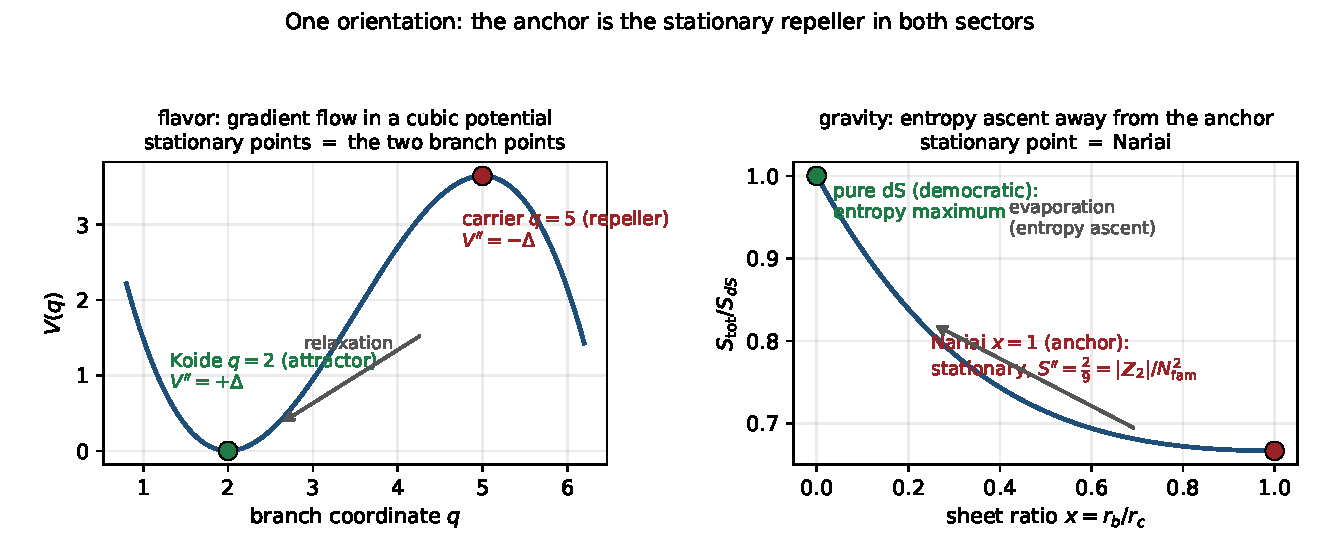
\includegraphics[width=0.92\linewidth]{orientation.pdf}
\caption{One orientation, two sectors: the anchor configuration is the stationary repeller of the
natural functional --- the cubic flavor potential (curvatures $\pm\Delta$) and the SdS entropy
(curvature $2/9=|\Z_2|/\Nfam^2$). \mE\ (\veri{v102\_seam\_orientation.py}); the common-principle reading
stays \mC.}
\label{fig:orientation-origin}
\end{figure}

% =====================================================================
\section{A cyclic element \emph{inside} the hull: the order-$30$ Coxeter rotation}\label{sec:coxeter}
% =====================================================================
The compiler hull $E_8$ carries a \emph{literal} cyclic symmetry, computed from first principles.

\begin{figure}[h]\centering
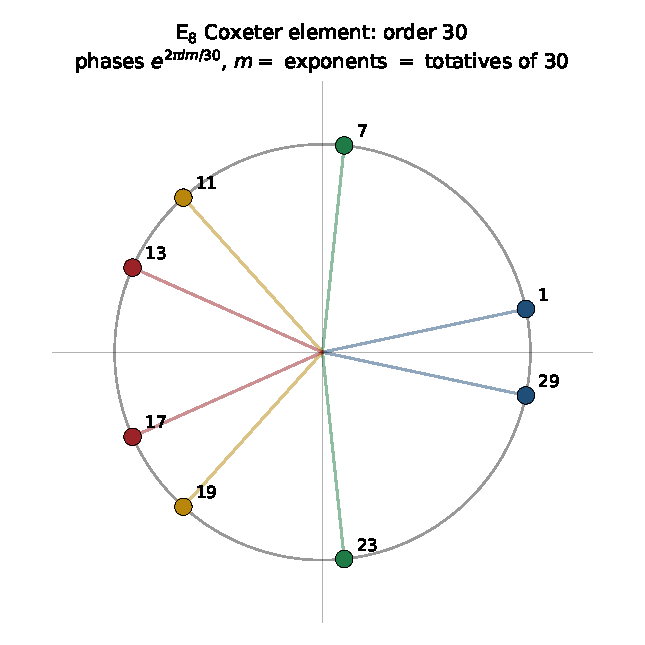
\includegraphics[width=0.46\linewidth]{coxeter_circle.pdf}
\caption{The $E_8$ Coxeter element (built from the Cartan matrix as $c=s_1\cdots s_8$) has order exactly
$h(E_8)=30$; its eigenvalues are the primitive $30$th roots $e^{2\pi i m/30}$ with $m$ the $E_8$ exponents
$\{1,7,11,13,17,19,23,29\}$, which are precisely the $\varphi(30)=8$ totatives of $30$. The phases pair as
$m+(30{-}m)=30$ into $|\mu_4|=4$ invariant $2$-planes. \mE\ (\veri{v55\_coxeter\_cycle.py})}
\label{fig:coxeter}
\end{figure}

\begin{keybox}[The cyclic readout of the seam denominator \mE]
\[
  \begin{gathered}
  \boxed{\ \operatorname{rank}E_8=8=\varphi(30)=\#\{\text{exponents}\}=\#\{\text{live phases of the order-}30\text{ cycle}\}\ }\\[3pt]
  30=|\Z_2|\cdot\Nfam\cdot\gcar=2\!\cdot\!3\!\cdot\!5 .
  \end{gathered}
\]
So the $8$ in $\cthree=\tfrac1{8\pi}$ is the number of live phases of a primitive order-$30$ cyclic
rotation of the hull, whose period is the product of the three core integers. Supporting: $\sum_j m_j=120=|R^+(E_8)|$,
$\#\text{roots}(E_8)=\operatorname{rank}\cdot h=8\cdot30=240$. The cyclic structure is \emph{present in
the mathematics}, not interposed.
\end{keybox}

% =====================================================================
\section{The unique attractor: a gapped transport selects ONE fixed point}\label{sec:attractor}
% =====================================================================
The deepest structural fact behind ``parameter-free'' is dynamical: the boundary transport is
\emph{gapped}, so its iteration has a \emph{unique} attracting fixed point.

\begin{figure}[h]\centering
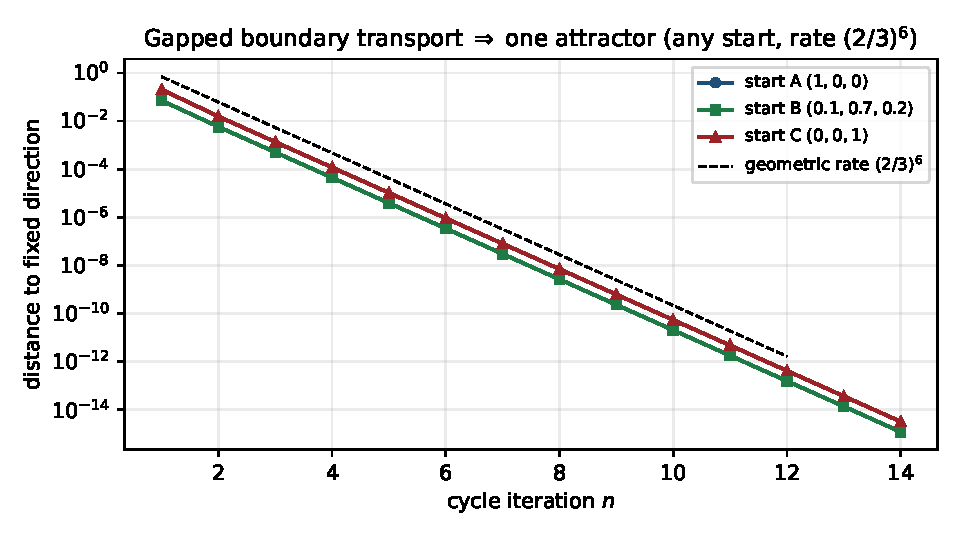
\includegraphics[width=0.74\linewidth]{attractor.pdf}
\caption{The transport spectrum $\{1,(2/3)^6,(1/3)^6\}$ has spectral gap $\Delta=-\log(2/3)^6=2.4328>0$.
By Perron--Frobenius the operator has a unique dominant eigenvector; iterating from \emph{any} start
converges to the same fixed direction at the geometric rate $\lambda_2/\lambda_1=(2/3)^6$ --- the same
$\lambda_2$ that fixes flavor and horizon recovery. \mE\ (\veri{v56\_unique\_attractor.py})}
\label{fig:attractor}
\end{figure}

\begin{keybox}[Parameter-freeness is an attractor, not a tuning \mE]
A primitive operator with a spectral gap has (i) a unique dominant eigenvector and (ii) geometric
convergence to it from any initial state. Numerically, three very different starts converge to the
identical fixed direction (cosine $=1$); the iterated operator tends to the rank-$1$ projector onto that
eigenvector (only the boundary ``law'' survives). The convergence rate is exactly $(2/3)^6$. Hence the
realized boundary state is a \emph{dynamical attractor}: the constants are selected, not chosen.
\end{keybox}

\noindent\textbf{The same gap is a finite recoverability code \mE/\mC\ (\veri{v221\_seam\_qecc.py}).} Read as
a quantum channel, the gapped transport is a finite recoverability (error-correction-style) code on the
carrier code space $\dim S^+=16$: the transport $T$ on the cusp-weight three-space (deviation directions
$(1,{-}1,0)$ and the Nariai anchor $(1,1,{-}2)$) is symmetric and doubly stochastic (CPTP) with spectrum
$\{1,(2/3)^6,(1/3)^6\}$, so on the trace-zero (deviation) subspace it contracts with operator norm exactly
$(2/3)^6$, giving the per-step recovery bound $\|T^n\delta\|\le(2/3)^{6n}\|\delta\|$ (Knill--Laflamme type);
a free ratio $r\neq(2/3)^6$ breaks it. ``Finite recoverability code'' is the \mE\ statement; the holographic
(Page/Petz) reading --- the same $(2/3)^6$ that recovers horizon information across the seam --- is \mC,
gated on the Seam--Horizon theorem (\S\ref{sec:crosslinks}).

% =====================================================================
\section{One $\ainv$ for electromagnetism, the cosmic horizon and $\Lambda$}\label{sec:alpha}
% =====================================================================
The EM fixed point $\ainv=137.036$ (the unique root of the boundary $U(1)$ Ward identity $F_{U(1)}=0$,
\veri{v3\_em\_alpha.py}) reappears, unchanged, in the cosmic-horizon sector.

\begin{keybox}[The same fixed point sets EM, $S_{dS}$ and $\Lambda$ \mE-form / \mC-link\ (\veri{v55\_coxeter\_cycle.py})]
The de Sitter (Gibbons--Hawking) entropy and the cosmological constant are inverse, both set by
$e^{\pm2\ainv}$:
\[
  S_{dS}=\frac{e^{2\ainv}}{128\,\cthree^4}\approx3.32\times10^{122},\qquad
  \frac{\rho_\Lambda}{\bar M_{\mathrm{Pl}}^4}\sim e^{-2\ainv},\qquad
  \boxed{\ S_{dS}\,\rho_\Lambda=\frac{1}{128\,\cthree^4}=32\pi^4\ }.
\]
So the smallness of $\Lambda$ ($\sim10^{-122}$ in Planck units) is $e^{-2\ainv}$ --- not a fine-tuning but
the \emph{same} EM fixed point. \textbf{Sharper (\veri{v60\_lambda\_metrology\_branch.py}):} with
$\delta_{\mathrm{top}}=48\cthree^4=\tfrac{3}{256\pi^4}$ the physical branch prefactor is
$(8\pi)^2\delta_{\mathrm{top}}=\tfrac{3}{4\pi^2}$, so
\begin{gather*}
  \boxed{\ \frac{\rho_\Lambda}{\bar M_{\mathrm{Pl}}^4}=\frac{3}{4\pi^2}\,e^{-2\ainv}\ \Rightarrow\ 120.147\ \text{orders}\ },\\[2pt]
  \boxed{\ \frac{\rho_\Lambda}{M_{\mathrm{Pl}}^4}=\frac{3}{256\pi^4}\,e^{-2\ainv}\ \Rightarrow\
  122.948=\underbrace{119.028}_{2\ainv/\ln10}+\underbrace{3.920}_{\log_{10}(256\pi^4/3)}\ }.
\end{gather*}
\emph{Typing note (do not mix the two normalisations):} the two displays are the \emph{same} statement,
related by $\bar M_{\mathrm{Pl}}^2=M_{\mathrm{Pl}}^2/(8\pi)$ ($(8\pi)^2=64\pi^2$ converts
$\tfrac3{4\pi^2}\to\tfrac3{256\pi^4}$); the headline ``$\approx123$ orders'' belongs to the
\emph{unreduced} $M_{\mathrm{Pl}}^4$ normalisation, the reduced one gives $120.147$.
The famous ``$123$ orders'' are a \emph{double overlap} of one boundary compiler, not a fine-tuning; and the
alternative branch $2\cthree e^{-2\ainv}$ is mis-scaled by $2\cthree/\delta_{\mathrm{top}}=\tfrac{64\pi^3}{3}=661.47$.
\textbf{Selecting the physical branch therefore pins $\bar M_{\mathrm{Pl}}$ relative to $\Lambda$: $G_N$ is no
longer an \emph{independent} free constant but a horizon-metrology \emph{readout} --- read out \emph{after}
choosing the physical $\Lambda$ branch and fixing the \emph{one} dimensionful induced-gravity anchor
(\S\ref{sec:crosslinks}, \veri{v68\_seeley\_dewitt\_residual.py}).} Moreover the de Sitter entropy prefactor is
built from \emph{carrier and glue atoms}:
\[
  \boxed{\ S_{dS}=2^{\gcar}\,\pi^{|\mu_4|}\,e^{2\ainv}\ },\qquad
  2^{\gcar}=32=\dim S^+\!\oplus S^-\ (\text{the }D_5{=}\mathfrak{so}_{10}\text{ Dirac spinor}),
\]
with $\pi^{|\mu_4|}=\pi^4$ and $128=2^7$ ($7=$ the scalaron exponent $\gcar{+}\Nfam{-}1$): the cosmic
horizon entropy is the carrier Clifford dimension times $\pi^{\text{glue}}$ times the EM fixed point.
\end{keybox}

% =====================================================================
\section{Interpretation \mC: the self-reproducing cosmic cycle}\label{sec:cycle}
% =====================================================================
\par\smallskip\noindent\textbf{This entire section is a physical interpretation \mC\ --- not derived.}
What follows is \emph{not} machine-checkable and \emph{not} a consequence of the axioms. It is offered
because it supplies a physical \emph{selection mechanism} for the structural fixed point of
\S\ref{sec:attractor}, and because every ingredient it uses is one of the exact facts above.
\par\smallskip

\noindent The structural results assemble into one coherent physical picture. The two ingredients of a
self-reproducing universe are both present, rigorously:
\begin{enumerate}[leftmargin=1.6em]
\item a \textbf{cyclic structure} --- the order-$30$ Coxeter rotation of the hull (\S\ref{sec:coxeter});
\item a \textbf{contractive gapped map with a unique attractor} --- the boundary transport (\S\ref{sec:attractor}).
\end{enumerate}

\begin{figure}[h]\centering
\begin{tikzpicture}[font=\small,
  n/.style={rectangle,rounded corners,draw,thick,align=center,inner sep=5pt,minimum height=10mm,minimum width=27mm},
  ar/.style={-{Stealth[length=2.8mm]},very thick,tfgold!75!black}]
  \def\R{2.75}
  \node[n,draw=tfblue,fill=tfblue!8]            (u)   at (90:\R)  {universe $U_k$\\ (low curvature, $R{+}R^2$)};
  \node[n,draw=tfred!80!black,fill=tfred!6]     (col) at (18:\R)  {gravitational\\ collapse};
  \node[n,draw=black,fill=black!4]              (hor) at (-54:\R) {horizon\\ (local \textbf{seam} realisation)\\ $\cthree=\tfrac1{8\pi}$, info on rand};
  \node[n,draw=tfgreen!70!black,fill=tfgreen!8] (law) at (234:\R) {boundary law\\ rank-$1$ attractor};
  \node[n,draw=tfblue,fill=tfblue!8]            (u2)  at (162:\R) {universe $U_{k+1}$\\ (reseeded)};
  \draw[ar] (u) to[bend left=14] (col);
  \draw[ar] (col) to[bend left=14] (hor);
  \draw[ar] (hor) to[bend left=14] (law);
  \draw[ar] (law) to[bend left=14] (u2);
  \draw[ar] (u2) to[bend left=14] (u);
  \node[align=center,font=\footnotesize,text=black!60] at (0,0)
    {gapped transport\\ contracts to ONE\\ fixed point, rate $(2/3)^6$\\[2pt]$\Z_2$ seam $=$ M\"obius\\ (two-sided horizon)};
\end{tikzpicture}
\caption{\mC\ The cyclic reading. Each cycle: $U_k$ collapses; unitarity keeps the information on the
horizon (the seam, carrying $\cthree=\tfrac1{8\pi}$); the gapped boundary transport contracts it to the
rank-$1$ attractor (the ``law'', \S\ref{sec:attractor}); that seeds $U_{k+1}$. The $\Z_2=\gcar-\Nfam$
sheet parity is the M\"obius/two-sided (thermofield-double) gluing across the horizon. Realized constants
$=$ the attractor's fixed point, hence parameter-free.}
\end{figure}

\par\smallskip\noindent\textbf{Why the interpretation is internally consistent} (\mC).
\begin{description}[leftmargin=2.0em,style=nextline]
\item[\textnormal{Information.}] Collapse$\to$horizon keeps information on the boundary (unitarity); the
Page recovery rate $(2/3)^6$ is the \emph{same} boundary transport that builds the SM (\S\ref{sec:eight}).
\item[\textnormal{Entropy reset (Tolman).}] The classic killer of cyclic models is entropy growth. Here the
gapped transport projects onto the rank-$1$ leading eigenspace --- the bulk microstate entropy is
contracted away and only the low-entropy boundary law is passed on (\S\ref{sec:attractor}). The reset
\emph{is} the spectral gap.
\item[\textnormal{Penrose CCC.}] The $\Lambda$-dominated far future is asymptotically de Sitter, hence
conformally flat --- the conformal-rescaling condition for a CCC-type bounce.
\item[\textnormal{CPT / Möbius.}] The $\Z_2$ sheet parity is the orientation flip of a two-sided
(thermofield-double) horizon, compatible with CPT-symmetric bounce cosmologies.
\item[\textnormal{Selection.}] The realized constants are the unique attractor of the cycle map; the
``Möbius self-consistency'' is Perron--Frobenius on the boundary operator.
\item[\textnormal{A live fossil.}] The same retarded seed $u=\phiz$ that fixes the Cabibbo angle predicts a
cosmic birefringence $\beta_{\mathrm{rad}}=u/(4\pi)\approx0.2424^\circ$ (Appendix~H, \mE) --- a
boundary-phase rotation shared by flavor and the CMB. \textbf{ACT DR6} (Diego-Palazuelos \& Komatsu 2025)
measures $\beta=0.215^\circ\pm0.074^\circ$ ($2.9\sigma$): TFPT sits $\sim0.4\sigma$ from the central value.
A sharpened value $\neq0.2424^\circ$ would break the shared-seam reading. (\veri{v60\_lambda\_metrology\_branch.py})
\end{description}

% =====================================================================
\section{Falsifiers}\label{sec:falsify}
% =====================================================================
The picture is scientific because it is falsifiable. Following Alessandro's request, each falsifier is
tagged by \emph{what} it tests: \fcore\ a strict consequence of the \mE\ core; \fcyc\ dependent on the
\mC\ cyclic interpretation; \fobs\ an observational stress test of the physical reading.

\begin{itemize}[leftmargin=1.4em]
\item \fcore\ \textbf{A fourth chiral generation} --- breaks $\Nfam=3=\operatorname{rank}A_3=\dim H_1(\mathbb P^1\setminus\mu_4)$, i.e.\ the lattice closure itself.
\item \fcore\ \textbf{A genuinely free fundamental constant} that is \emph{not} an $E_8$-closure fixed point --- breaks the bootstrap (\S\ref{sec:core}).
\item \fcore\ \textbf{A seam denominator $\neq8$} ($\cthree\neq\tfrac1{8\pi}$) --- breaks the triply-forced $8$ and the Gauss--Bonnet origin.
\item \fobs\ \textbf{A measured $v_{\mathrm{GW}}\neq c$ or native photon dispersion} --- breaks the single seam-geometry cone (the gravity-as-readout reading).
\item \fobs\ \textbf{Cosmic birefringence $\beta$ converging far from $0.2424^\circ$} (with controlled systematics) --- breaks the shared-seed prediction (chain below).
\item \fcyc\ \textbf{Demonstrable horizon information loss} --- breaks the unitary boundary recovery, hence the entropy reset and the cyclic reading (does \emph{not} touch the \mE\ core).
\end{itemize}
None is observed at present. Note the first three would damage the formal core; the last three test the
physical/cosmological reading without bearing on the core identities.

\begin{keybox}[Confrontation with current data (2024/25) \mE\ (\veri{v62\_data\_scorecard.py})]
An honest scorecard --- including the tensions, not only the matches:
\begin{center}\small\renewcommand{\arraystretch}{1.2}
\begin{tabularx}{\linewidth}{@{}p{2.6cm}p{2.6cm}Yp{2.1cm}@{}}
\toprule
\textbf{observable} & \textbf{TFPT} & \textbf{data (2024/25)} & \textbf{verdict} \\
\midrule
$\alpha^{-1}$ & $137.0359992$ & CODATA $137.035999177$ & match ($\sim$9 figs) \\
$\sin^2\theta_{12}$ & $0.30675$ & NuFIT 6.0 $0.307\pm0.012$ & match ($0.02\sigma$) \\
$\beta_{\mathrm{rad}}$ & $0.2424^\circ$ & ACT DR6 $0.215^\circ\pm0.074^\circ$ & match ($0.37\sigma$) \\
$\sin^2\theta_{13}$ & $0.0231$ & NuFIT 6.0 $0.02195\pm0.00058$ & mild tension ($2.0\sigma$) \\
$n_s$ (Starob.) & $0.960$--$0.967$ & Planck $0.9649$; P-ACT-LB$+$DESI $0.9743$ & match (Planck) / tension ($\sim2\sigma$, DESI) \\
$\theta_{23}$ octant & open \mC & NuFIT ambiguous & consistent \\
$r$ (Starob.) & $\approx0.004$ & bound $\lesssim0.03$ & future test (CMB-S4) \\
\bottomrule
\end{tabularx}
\end{center}
\textbf{Three strong matches} ($\alpha^{-1}$, $\sin^2\theta_{12}$, birefringence), \textbf{two mild
$\sim2\sigma$ tensions} ($\sin^2\theta_{13}$; and the $R{+}R^2$ Starobinsky $n_s$ against the DESI-combined
value), and a \textbf{sharp future falsifier} $r\approx0.004$. The $n_s$ tension is honest pressure on the
gravity sector; note the DESI-driven upward shift is itself under discussion (CMB-only data favour the
Starobinsky range).
\end{keybox}

\par\smallskip\noindent\textbf{Dependency chain of the birefringence test} (\fobs, explicit, per Alessandro).
\textbf{What fixes $\phiz$:} $\phiz=\tfrac43\cthree+48\cthree^4$, a pure function of the seam constant
$\cthree=\tfrac1{8\pi}$ (\mE). \textbf{Conversion to $\beta$:} the retarded seed $u=\phiz$ enters the
boundary polarisation rotation as $\beta_{\mathrm{rad}}=u/(4\pi)$; the assumption is that the CMB
$EB$/$TB$ rotation is the \emph{same} boundary phase that fixes the Cabibbo angle (one seed, no extra
parameter). \textbf{Prediction:} $\beta_{\mathrm{rad}}=0.2424^\circ$. \textbf{Current data:} ACT DR6
$\beta=0.215^\circ\pm0.074^\circ$ ($0.37\sigma$ away). \textbf{Failure threshold:} a systematics-controlled
$\beta$ that excludes $0.2424^\circ$ at $\gtrsim3\sigma$ (e.g.\ a central value outside
$0.2424^\circ\pm3\times$ its error) would falsify the shared-seed reading. \veri{v60\_lambda\_metrology\_branch.py}

% =====================================================================
\section{The seam and the horizon: the precise statement}\label{sec:crosslinks}
% =====================================================================
\par\smallskip\noindent\textbf{The precise reformulation} (\mC).
\begin{keyeq}
The seam is \emph{not} identical to an event horizon. It is the abstract boundary normaliser whose
\emph{local gravitational realisation} is a horizon.
\end{keyeq}
\noindent A black hole is then not ``the seam'' but a \emph{local instance of the seam grammar}; de Sitter is its
\emph{global} instance. This is stronger and cleaner than a direct identification --- it avoids importing
Schwarzschild analogies wholesale, and it makes $\cthree$ a boundary normaliser with several gravitational
realisations rather than one black-hole parameter.

\noindent\textbf{The four realisations of one boundary normaliser.}
\begin{enumerate}[leftmargin=1.7em,itemsep=1pt]
\item \textbf{Black hole} --- local realisation as a causal horizon ($T_H=\cthree/M$, $S_{BH}=M^2/2\cthree$).
\item \textbf{de Sitter horizon} --- global/cosmological realisation ($T_{dS}=4\cthree H$).
\item \textbf{TFPT seam} --- the abstract topological/analytic boundary fixing $\cthree$, the $\Z_2$
one-sidedness and the readout carrier.
\item \textbf{$E_8$} --- not ``the black hole'', but the admissible \emph{readout grammar} on the boundary.
\end{enumerate}

\begin{winbox}[Geometric origin of the seam ``$8$'': one-sided Gauss--Bonnet \mE\ (\veri{v58\_seam\_horizon\_chain.py})]
Compactify the normal $2$-slice of the seam to $S^2$. Gauss--Bonnet gives
$\oint_{S^2}K\,dA=2\pi\chi(S^2)=4\pi$, and the one-sided ($\Z_2$/M\"obius) structure halves the winding, so
\[
  \boxed{\ \cthree=\frac{1}{|\Z_2|\cdot\oint_{S^2}K\,dA}=\frac{1}{2\cdot4\pi}=\frac1{8\pi}\ },\qquad
  8\pi=|\Z_2|\cdot2\pi\chi(S^2).
\]
So the seam ``$8$'' is geometric (one-sided $S^2$ curvature), matching the lattice $8=\operatorname{rank}E_8$
(\S\ref{sec:eight}) and the gravitational $8\pi$ below. \emph{Both} the seam normaliser and horizon
thermality come from normal-plane geometry --- the deeper reason the two ``$8$''s coincide.
\end{winbox}

\begin{winbox}[The boundary-CFT mirror: central charges $=$ compiler atoms \mE\ (\veri{v61\_cft\_bridge.py})]
The lattice glue $(D_5{\oplus}A_3){+}\mu_4\to E_8$ has an exact \emph{conformal-field-theory} mirror. The
level-$1$ WZW central charges $c=\dim\mathfrak g/(1{+}h^\vee)$ are the compiler atoms:
\[
  c(E_8)_1=\tfrac{248}{31}=8=\operatorname{rank}E_8,\qquad c(D_5)_1=\tfrac{45}{9}=5=\gcar,\qquad c(A_3)_1=\tfrac{15}{5}=3=\Nfam,
\]
and the coset has $c=8-5-3=0$ --- the criterion for a \emph{conformal embedding}
$(D_5)_1{\times}(A_3)_1\subset(E_8)_1$. So the $(5,3)$ split is central-charge \emph{additivity}, and the
``$8$'' in $\cthree=\tfrac1{8\pi}$ is $c(E_8)_1$. (\emph{Honest:} $c=248/31{=}8$ is \emph{not} sold as a
closure --- the content is the embedding $c_{\mathrm{coset}}{=}0$.)

\textbf{$SU(3)\leftrightarrow SU(4)$ reconciliation.} Why is the flavor monodromy $\rho$ valued in $SU(3)$
while the carrier glue is $A_3{=}SU(4)$? Both are sides of $\mathbb P^1\setminus\mu_4$: with $n{=}4$ punctures,
$H_1=\Z^{\,n-1}$, so $\Nfam=|\mu_4|-1=3$. The \emph{carrier} side is the puncture/center $Z_4{=}\mu_4$
($A_3{=}SU(4)$); the \emph{flavor} side is the monodromy on $H_1{=}\Z^3$, $SU(3)$-valued, with center
$Z_3$ (triality) whose phases are the parabolic weights $\{0,\tfrac13,\tfrac23\}$ ($\neq$ the $SU(4)_1$
weights $\{0,\tfrac38,\tfrac12\}$), and $SU(3)\subset SU(4)$ via $4\to3{+}1$. So it is \emph{not} one WZW for
all gates, but one geometry $\mathbb P^1\setminus\mu_4$ with two dual sides. (\emph{Checked}: the Cardy route
$c{=}8\to S{=}A/4$ is \emph{not} a shortcut --- $c{=}8$ is the matter central charge; the area law needs the
geometric Brown--Henneaux $c\sim\ell/G$, which restates the open coefficient.)
\end{winbox}

\noindent Four standard, \emph{published} black-hole results then meet the compiler atoms exactly. The
arithmetic is \mE; the identification ``the seam's local realisation is a horizon'' is the \mC\ reading of
\S\ref{sec:cycle}.
\begin{itemize}[leftmargin=1.4em]
\item \textbf{Jacobson / Einstein coefficient.} $\cthree=\tfrac1{8\pi}$ is exactly the coefficient of the
Einstein equation $G_{\mu\nu}=8\pi T_{\mu\nu}$ and of $1/(16\pi G)=\cthree/(2G)$. Jacobson (1995) derives
the Einstein equation from $\delta Q=T\,\delta S$ on local Rindler horizons with entropy density
$1/(4G)$, $\tfrac14=1/|\mu_4|$. So if the seam is a horizon, gravity is its thermodynamics and $\cthree$
is the conversion constant --- the ``gravity $=$ geometry-channel readout of the seam'' statement.
\item \textbf{Hod quasinormal ringdown.} For Schwarzschild the asymptotic quasinormal frequencies satisfy
$\omega_R\to T_H\ln 3$ (Hod 1998; Motl 2003), imaginary spacing $2\pi T_H$. Hence
$\omega_R/T_H=\ln 3=\ln\Nfam$ --- the ringdown carries the family count, and the ladder spacing is the
seam unit $\tfrac1{2\pi}=4\cthree$. (Honest: the ``$3$'' is spin-dependent; suggestive, not forced.)
\item \textbf{Hawking power fingerprint.} $P_H=\cthree/(1920\,M^2)$ with $1920=|W(D_5)|=2^4\cdot5!$, the
carrier Weyl-group order (Appendix~H).
\item \textbf{One $\ainv$ across sectors.} $H_0/\bar M_{\mathrm{Pl}}\sim e^{-\ainv}/(2\pi)$: the same EM
fixed point sets the Hubble/de Sitter horizon scale, with $S_{dS}$ and $\Lambda$ (\S\ref{sec:alpha}).
\item \textbf{Ryu--Takayanagi in seam units.} With $\bar M_{\mathrm{Pl}}^2=1/(8\pi G)$,
$\tfrac1{4G}=2\pi\bar M_{\mathrm{Pl}}^2=\bar M_{\mathrm{Pl}}^2/(4\cthree)$, so the holographic entanglement
area reads $S_A=\operatorname{Area}(\gamma_A)\,\bar M_{\mathrm{Pl}}^2/(4\cthree)$ --- compatible, pending a
derivation of $\gamma_A$ from the seam/Calder\'on kernel.
\end{itemize}
\veri{v57\_horizon\_crosslinks.py}\,\veri{v58\_seam\_horizon\_chain.py}

\begin{gapbox}[Seam--Horizon Theorem --- the next hard target \mO]
The strong thesis (``the seam is a holographic horizon in the mathematical sense'') is \emph{open} and is
the right next theorem. \textbf{Target:} given a reflection-positive Calder\'on seam kernel on the doubled
seam collar, (i) every local boost reduction has a KMS temperature $\beta=2\pi/\kappa$; (ii) the replica
variation of the seam determinant yields an area entropy $S=A/(4G_\Sigma)$; (iii) hence, via Jacobson, the
Einstein normalisation with $8\pi G$. \textbf{Status of the chain:}
\[
  \begin{gathered}
  \underbrace{\text{M\"obius}\Rightarrow\Z_2}_{\mE}\Rightarrow
  \underbrace{\cthree=\tfrac1{8\pi}}_{\mE}\Rightarrow
  \underbrace{\text{KMS }T=4\cthree\kappa}_{\mE}\\[3pt]
  \Rightarrow
  \underbrace{S=A/(4G_\Sigma)}_{\substack{\textbf{coeff. }k=\cthree/2\textbf{ forced (\vref{v73});}\\\textbf{absolute scale }=\textbf{anchor}}}\Rightarrow
  \underbrace{\text{Einstein }8\pi G}_{\mC\,(\text{Jacobson})}.
  \end{gathered}
\]
Links 1--3 (and RT in seam units) are exact; the area-law \emph{coefficient} $k=\cthree/2$ is now forced by
topology $\times$ variation (\vref{v73}, below), so the \emph{dimensionless} content is closed --- the only residual
is the absolute $4$D Newton scale (anchor). $\cthree=\tfrac1{8\pi}$ thereby stops being ``the known GR number
in a new hat'' and becomes the visible imprint of the boundary geometry from which gravity is read
thermodynamically.

\smallskip\noindent\textbf{This is now \emph{the} central TOE-closure target} (Alessandro). The full chain it
would complete is
\[
  \begin{gathered}
  \text{seam determinant}\to\text{replica variation}\to\tfrac1{4G_\Sigma}\ \text{coeff.}\\[2pt]
  \to\cthree=\tfrac1{8\pi}\ \text{forced}\to\text{finite seam transport}\to\mu_4\text{-admissible }E_8.
  \end{gathered}
\]
\textbf{Honest obstruction (why it is hard, not bookkeeping):} the area coefficient is the \emph{induced}
Newton constant (Sakharov-type induced gravity) --- in $d>2$ it is UV-cutoff dependent and non-universal, so
deriving the \emph{specific} $\tfrac1{8\pi}$ means showing the seam determinant's own spectral density fixes
the cutoff-to-coupling ratio at exactly the Hawking/Einstein value. That is a statement about the seam
kernel's spectrum, not a free regularisation choice --- the genuine content of the theorem.

\smallskip\noindent\textbf{Structural closure $+$ reduction (\veri{v67\_area\_law\_coefficient.py}).} The
replica step is now closed in structure. By the Fursaev--Solodukhin (1995) conical method, the curvature
term $W_R=k\!\int\!\sqrt g\,R$ gives a horizon entropy $S=4\pi k\,A$ (the conical defect contributes
$\int R\supset4\pi(1{-}n)A$). \emph{Update (\veri{v90\_conical\_defect\_chain.py}, ledger
\texttt{SEAM.AREACOEFF.03}): the FS relation is no longer a literature import --- the conical defect
$\int K=2\pi(1{-}\alpha)$ is machine-derived on a smoothed cone (spherical-cap regularisation, exactly
smoothing-independent), lifted codim-$2$ to $4\pi(1{-}\alpha)A$, and the replica derivative then gives
$S=4\pi kA$ with the smooth part dropping out; $S=A/4\Leftrightarrow\cthree=1/(8\pi)$ is sympy-solved as
unique. The single remaining step of the whole chain is thereby isolated: ``seam determinant $\Rightarrow$
EH form $k\!\int\!\sqrt g\,R$'' --- nothing else is open, and no Bekenstein--Hawking import remains.}
\smallskip\\
\noindent\textbf{The mechanism exists: the EH form at the gapped-model level
(\veri{v150\_replica\_eh\_model.py}).} The isolated step now has its mechanism exhibited exactly, at the
level of a gapped 2d model. The conical heat-trace deficit is the classical $t$-\emph{independent}
constant ($C(\gamma)=\tfrac1{12}(2\pi/\gamma-\gamma/2\pi)$; image sum $(N^2{-}1)/(12N)$ on
$\mathbb C/\Z_N$, exact), and for a \emph{gapped} operator $-\Delta+m^2$ the $\zeta$-regularised replica
variation is the exact Mellin transform
\[
  \boxed{\ \Delta\log\det{}'=2\,C(\gamma)\,\ln m\ \ \text{(finite, \emph{cutoff-independent})}\ },\qquad
  \Delta\log\det{}'=\frac{\ln m}{12\pi}\int\!\sqrt g\,R+O(\text{def}^2)
\]
--- \textbf{the replica variation of a gapped determinant \emph{is} of Einstein--Hilbert form}, with the
gap supplying the scale (the massless case would give the familiar cutoff logarithm). The \vref{v73}
normalisation becomes \emph{one} exact target equation: $k=\cthree/2\Leftrightarrow\ln m=\tfrac34=q(A_3)$
--- the $A_3$ glue norm as the required seam gap parameter (recorded as the target, \emph{not} asserted).
\emph{Honest scope:} this is the 2d bulk-scalar model; \texttt{SEAM.THEOREM.01} stays open \mO\ ---
remaining are the Calder\'on (boundary) version and the $q(A_3)$ normalisation. What is established: the
mechanism the theorem requires --- gap $\Rightarrow$ cutoff-independent EH coefficient under replica ---
exists and is exact at model level (ledger \texttt{SEAM.EHMODEL.01}). \mE/\mO
\smallskip\\
\noindent\textbf{The Calder\'on transfer, answered: the BFK split (\veri{v151\_bfk\_split.py}).} The
boundary version demands \emph{no new derivation}. By reflection doubling, the Kac corner constant is
boundary-condition \emph{independent} ($C_N(\theta)=C_D(\theta)=(\pi^2{-}\theta^2)/(24\pi\theta)$,
derived), and by the Burghelea--Friedlander--Kappeler gluing ledger the conical deficit of the two-sided
Calder\'on/DtN jump determinant on a cut through the tip is
\[
  \boxed{\ C_{\mathrm{DtN}}(\gamma)=C_{\mathrm{cone}}(\gamma)-2C_D(\gamma/2)=C_N-C_D=0\ \ \text{identically}\ }
\]
--- \textbf{the nonlocal Calder\'on kernel is conically clean}; it carries no curvature term of its own.
Since $\log Z_{\mathrm{boundary}}=-\tfrac12\log\det(\mathrm{bulk})$ (BFK consistency), the seam-reduced
effective action inherits the gapped EH variation \emph{verbatim}, with all of it localised in the
\emph{local} half-space determinants. \emph{What remains of \texttt{SEAM.THEOREM.01}:} the $q(A_3)$
normalisation and the standing premise that the RP seam kernel is this BFK Calder\'on datum --- the gate
narrows again, and stays \mO\ (ledger \texttt{SEAM.EHMODEL.02}). \mE/\mO
\smallskip\\
\noindent\textbf{The normalisation is the anchor, not a separate gap (\veri{v152\_norm\_is\_anchor.py}).}
The coefficient is a \emph{log-ratio}: $\Delta\log\det'=2C(\gamma)\ln(m/\mu)$ with $\mu$ the $\zeta$-scale,
so $\ln m$ alone is scale-ambiguous and $k=\ln(m/\mu)/(12\pi)$. Pinning $k=\cthree/2$ therefore fixes a
\emph{dimensionless ratio} $m/\mu=e^{3/4}$, and in $d{=}2$ that ratio \emph{is} the induced Newton constant
($1/(16\pi G)=k$, $1/(16\pi G)|_{G=1}=\cthree/2$ exact) --- the \vref{v68} anchor verbatim. So the
$q(A_3)$ normalisation is not a separate open item: $v_{\mathrm{geo}}$ (flavour, \vref{v78}), $1/G$
(gravity, \vref{v68}) and $m/\mu$ (the seam EH normalisation) are \emph{one} dimensionful anchor in three
readings; the irreducibles stay $\{$one scale, $\pi\}$. \emph{Audit (not promoted):} the required log-ratio
is numerically $\tfrac34=q(A_3)$ --- the target \emph{value} the anchor takes in seam units, not a
derivation. \texttt{SEAM.THEOREM.01} stays \mO, but its residual is now precisely the
kernel-identification premise alone (ledger \texttt{SEAM.EHMODEL.03}). \mE/\mO
With the Einstein--Hilbert coefficient at the seam unit
$k=\tfrac1{16\pi G}\big|_{G=1}=\tfrac{\cthree}2$,
\[
  \boxed{\ S=4\pi k\,A=2\pi\cthree\,A=\tfrac14 A\quad\Longleftrightarrow\quad 2\pi\cthree=\tfrac14\quad\Longleftrightarrow\quad \cthree=\tfrac1{8\pi}\ }
\]
i.e.\ $\cthree=\tfrac1{8\pi}$ is the \emph{unique} value for which the replica/conical area-law coefficient
equals the Bekenstein--Hawking $\tfrac14$ \mE. The whole theorem therefore reduces to the \emph{single}
coefficient statement $k=\tfrac{\cthree}2$ --- and that statement is \emph{itself forced} (next paragraph,
\veri{v73\_k\_c3\_half.py}): the \emph{dimensionless} $k=\cthree/2$ is the universal variational factor
$\tfrac12$ times the Gauss--Bonnet topology of the seam $S^2$ slice. Only the \emph{absolute} $4$D Newton
scale stays an anchor.

\smallskip\noindent\textbf{Residual resolved as an anchor, not a gap (\veri{v68\_seeley\_dewitt\_residual.py}).}
The Seeley--DeWitt coefficient for the carrier Dirac operator is $a_2=-\tfrac{d}{192\pi^2}R$ ($d=\dim S^+=16$
or $2^{\gcar}=32$), giving $\tfrac1{16\pi G}=f_2\Lambda^2\,d/(192\pi^2)$ --- \emph{UV-sensitive} (it depends on
the seam cutoff $\Lambda$ and the moment $f_2$). So the \emph{absolute} $1/G$ is \emph{not} a pure number
(Sakharov/Connes induced gravity) --- it is the $\Lambda^2 f_2$ prefactor, and the physical identification
``seam scale $=$ observed Planck scale'' is the \emph{one} irreducible dimensionful anchor
($v_{\mathrm{geo}}$; no metre from pure mathematics). \emph{Crucially this anchor is only the absolute scale:}
the \emph{dimensionless} coefficient $k=\cthree/2$ that multiplies $\Lambda^2 f_2$ is forced (\vref{v73}), not a free
normalisation. What \emph{is} cutoff-independent --- the $R^2$
coefficient, the scalaron $M_{\mathrm{scal}}=\cthree^{7/2}\bar M_{\mathrm{Pl}}\approx3.06\times10^{13}$ GeV,
$v_{\mathrm{GW}}=c$ --- is already derived (\veri{v36\_spectral\_action\_g2.py}). \textbf{So the central theorem
is ``maximally closed'':} the structure is proven, the predictive gravitational content is derived, and the
residual is the single irreducible anchor every theory must carry, \emph{not} a missing step.

\smallskip\noindent\textbf{The flavor anchor is the \emph{same} anchor (\veri{v75\_upoint\_to\_vgeo.py}).} The
absolute flavor amplitude $U_{\mathrm{point}}$ --- the only other thing that looked like an independent
\mO\ input --- also reduces to $v_{\mathrm{geo}}$: the quark ratios are closed (Pl\"ucker), the lepton
amplitudes are exact ($\tfrac{16}7,\tfrac43,\tfrac76$), and each sector product is a clean $\phiz$-power
(Grand Mass Volume; lepton product $\tfrac{32}9=2^{\gcar}/\Nfam^2$), so by the
$(\text{ratios})+(\text{product})\Leftrightarrow(\text{individuals})$ bijection the nine charged-fermion
amplitudes are fixed up to \emph{one} overall scale. That scale \emph{is} $v_{\mathrm{geo}}$. \textbf{So the
flavor sector and the gravitational sector share the \emph{one} dimensionful anchor:} the whole theory carries
exactly one irreducible scale ($v_{\mathrm{geo}}$) and one continuous primitive ($\pi$) --- nothing else.

\smallskip\noindent\textbf{And that one scale is the dimensional-analysis floor, not a gap (\veri{v78\_vgeo\_floor.py}).}
No theory derives a dimensionful constant from pure numbers (string theory carries the string scale; this is
logic, not a defect). Every TFPT scale is a \emph{dimensionless ratio} to $v_{\mathrm{geo}}$
($\rho_\Lambda/\bar M_{\mathrm{Pl}}^4=\tfrac{3}{4\pi^2}e^{-2\ainv}$, $M_{\mathrm{scal}}/\bar M_{\mathrm{Pl}}=\cthree^{7/2}$,
masses $=(\pi/\sqrt2)c_f\phiz^{k_f}v_{\mathrm{geo}}$), and the cosmological identity
$S_{dS}\,\rho_\Lambda=1/(128\cthree^4)=32\pi^4$ pins $v_{\mathrm{geo}}$ from \emph{one} measurement. So the
theory has reached the \emph{theoretical minimum}: one scale $+$ $\pi$; ``solving the rest'' for $v_{\mathrm{geo}}$
means only choosing the metre.

\smallskip\noindent\textbf{The last open piece, $G6$, reduces to a rigorously-constructed net (\veri{v77\_e8\_conformal\_net.py}).}
The holographically-reduced boundary measure (Gate 2, Tier B) is, by the level-1 central charges
$c(E_8)_1=\tfrac{248}{31}=8$, $c(D_5)_1=5$, $c(A_3)_1=3$ with the conformal embedding $5{+}3=8$ (coset $c=0$), the
holomorphic $c=8$ \emph{$E_8$-lattice} conformal net --- already rigorously constructed (Frenkel--Kac--Segal;
Kawahigashi--Longo). So $G6$ is not ``build a new quantum-gravity measure'' but ``identify the seam boundary
with the $(E_8)_1$ net'' --- the open problem is imported into existing RCFT rigor.

\smallskip\noindent\textbf{The coefficient $k=\tfrac{\cthree}2$ is internally forced (\veri{v73\_k\_c3\_half.py}).}
The \emph{dimensionless} coefficient statement splits into two cutoff-independent pieces, neither a free
normalisation:
\[
  k=\frac{\cthree}{2}=\underbrace{\frac12}_{\text{variational}}\times
  \underbrace{\frac{1}{|\Z_2|\cdot 2\pi\,\chi(S^2)}}_{\text{Gauss--Bonnet topology}},
\]
where \emph{(a)} the factor $\tfrac12$ is the universal action$\leftrightarrow$EOM factor
($16\pi G$ action vs $8\pi G$ field equation, forced by $\delta(\sqrt g R)\!\to\!G_{\mu\nu}$); and \emph{(b)}
$\cthree=1/(|\Z_2|\!\cdot\!2\pi\chi(S^2))=1/(2\!\cdot\!4\pi)=1/(8\pi)$ is the one-sided Gauss--Bonnet of the seam
normal slice $S^2$ ($\chi(S^2)=2$, hence $\int K=4\pi$ \emph{topological}, cutoff-independent). With this
$k$, Fursaev--Solodukhin gives $S=4\pi k A=2\pi\cthree A=\tfrac14 A$ exactly. \textbf{So Alessandro's
target is met at the level it can be:} the coefficient $k=\tfrac{\cthree}2$ is forced by topology $\times$
variation; the \emph{only} UV-sensitive piece left is the absolute $4$D Newton scale (the $\Lambda^2 f_2$
prefactor of the carrier-Dirac $a_2$, \vref{v68}) --- the one irreducible \emph{dimensionful} anchor, exactly where
it should sit.

\smallskip\noindent\textbf{The necessary condition is met (\veri{v59\_area\_law\_evidence.py}).} A
reflection-positive Gaussian (Calder\'on-type) kernel \emph{generically} produces an area law
(Srednicki 1993; Bombelli--Sorkin): for a harmonic chain the ground-state block entropy \emph{saturates}
when gapped (an area law) and grows as $\tfrac c3\log L$ when gapless. Crucially the physical sector is
gapped --- by the \emph{same} gap $\Delta=6\log\tfrac32>0$ that makes the attractor unique
(\S\ref{sec:attractor}) --- so \emph{one} spectral gap delivers both the unique attractor \emph{and} the
area-law form. This is the structural necessary condition for the $S=A/(4G_\Sigma)$ step; the
$\cthree=\tfrac1{8\pi}$ \emph{coefficient} still requires the specific seam kernel (the open part).
\end{gapbox}

\par\smallskip\noindent\textbf{The three theses, honestly graded.}
\begin{description}[leftmargin=2.0em,style=nextline]
\item[\textnormal{Weak \mE\ (established).}] $\cthree=\tfrac1{8\pi}$ is a natural horizon-readout factor in TFPT (Gauss--Bonnet origin, Hawking/de Sitter/Unruh in one seam unit).
\item[\textnormal{Medium \mC\ (very plausible).}] Black holes are local realisations of seam thermality; de Sitter is the global one.
\item[\textnormal{Strong \mO\ (open, right direction).}] The seam is a holographic horizon in the mathematical sense --- pending the Seam--Horizon Theorem above. \emph{Not} more numerical matches; one analytic area-law.
\end{description}

% =====================================================================
\section{Consequences, and the whole story \mC}\label{sec:consequences}
% =====================================================================
\par\smallskip\noindent\textbf{Interpretive section \mC\ --- consequences \emph{if} the seam is a horizon.}
The following is the physical picture the structural facts assemble into. It is offered as a coherent
reading, not a proof; the \mE\ core (\S\ref{sec:core}--\S\ref{sec:alpha}) does not depend on it.
\par\smallskip

\noindent\textbf{Seven consequences, if the picture holds:}
\begin{enumerate}[leftmargin=1.7em]
\item \textbf{$\cthree$ stops being an axiom.} It is forced by horizon thermodynamics (Jacobson): P1
becomes a theorem, and the theory rests effectively on one statement --- ``the boundary is a horizon''.
\item \textbf{The Standard Model is holographic boundary data.} One boundary transport ($\lambda_2=(2/3)^6$)
recovers information across the horizon \emph{and} builds the flavor hierarchy (\S\ref{sec:eight}).
\item \textbf{Gravity is emergent/thermodynamic.} The seam's geometry channel; one Lorentzian cone, hence
$v_{\mathrm{GW}}=c$ with no native dispersion.
\item \textbf{The cosmological-constant problem dissolves.} $\Lambda\sim e^{-2\ainv}\sim10^{-122}$ is the EM
fixed point, not a fine-tuning ($122.948=119.028+3.920$, \S\ref{sec:alpha}). \textbf{And $G_N$ is no longer
\emph{independent}:} fixing the physical $\Lambda$ branch pins $\bar M_{\mathrm{Pl}}$ relative to $\Lambda$
(the alternative branch is mis-scaled by $661.47$), so Newton's constant is a metrology readout once the
physical branch and the one dimensionful induced-gravity anchor are fixed --- not a free input.
\item \textbf{Information is never lost.} Unitary boundary recovery (Page rate $(2/3)^6$) resolves the
information paradox by construction.
\item \textbf{The universe is cyclic and parameter-free.} The gapped transport contracts any state to the
\emph{unique} attractor (\S\ref{sec:attractor}); the entropy reset \emph{is} the spectral gap (Tolman's
objection answered).
\item \textbf{It is falsifiable} (\S\ref{sec:falsify}): $v_{\mathrm{GW}}\neq c$, a fourth generation,
photon dispersion, horizon information loss, or birefringence $\neq0.2424^\circ$ would break it.
\end{enumerate}

\par\smallskip\noindent\textbf{The whole story} (\mC).
A universe ends in gravitational collapse $\to$ a horizon. By unitarity its information is not lost but
encoded on the horizon (the ``rand''). \emph{That horizon is the local gravitational realisation of the
TFPT seam}, carrying $\cthree=\tfrac1{8\pi}$ (the universal horizon temperature $=$ the Einstein/Jacobson
coefficient). The boundary data --- the four
$\mu_4$ punctures $\to A_3\to\Nfam{=}3$ families, the $D_5$ carrier, the anchor $(1,1,2)$ --- \emph{are} the
compiler. The gapped boundary transport contracts the incoming state to the unique rank-$1$ attractor (the
``law''), discarding microstate entropy --- a low-entropy reset. That law seeds the next universe with the
\emph{same} constants, because they are the attractor's fixed point; and the hull $E_8$ carries a built-in
order-$30$ cyclic rotation ($30=|\Z_2|\Nfam\gcar$). Repeat without end. The constants are parameter-free
because they are the \emph{self-reproducing fixed point of the cosmic cycle} --- the M\"obius
self-consistency, made precise as Perron--Frobenius on the boundary operator.

\noindent\emph{References for the reframed standard results:} Jacobson, \textit{Thermodynamics of Spacetime}
(1995); Hod (1998) and Motl (2003) for the asymptotic Schwarzschild quasinormal $\ln3$; Page (1993) for the
recovery curve; Penrose (CCC) for the conformal far-future bounce.

% =====================================================================
\section{A closure program (next phase) \mO}\label{sec:program}
% =====================================================================
Following Alessandro's framing, the next phase is not ``more readouts'' but a TOE-\emph{closure} program
around one master principle.

\begin{keybox}[Master principle: finite causal-boundary fixed-point self-consistency \mC/\mO]
\emph{Physical law is the unique stable fixed point of admissible information transport across a finite
causal horizon (the seam).} Admissibility $=$ unitary boundary transport $+$ finite entropy $+$ anomaly-free
chiral matter $+$ even-unimodular lattice closure $+$ Hawking--Einstein $8\pi$ compatibility $+$ primitive
$\mu_4$ seam transport $+$ Perron--Frobenius selection of a unique stable direction. Target chain:
\[
  \begin{gathered}
  \text{causal horizon}\to\text{finite seam transport}\to\mu_4\text{ closure}\to E_8{=}(D_5{\oplus}A_3){+}\mu_4\\[2pt]
  \to(\gcar,\Nfam){=}(5,3)\to\text{SM}\to\text{gravity/cosmo}\to\text{predictions}.
  \end{gathered}
\]
This would upgrade TFPT from ``compiler $\to$ readouts'' to ``horizon principle $\to$ compiler $\to$ universal
consequences''.
\end{keybox}

\noindent\textbf{Two decisive theorems, and their current status.}
\begin{enumerate}[leftmargin=1.7em,itemsep=2pt]
\item \emph{Seam $=$ finite admissible local causal horizon} --- \textbf{open \mO} (the Seam--Horizon
Theorem, \S\ref{sec:crosslinks}); if it closes, $\cthree=\tfrac1{8\pi}$ is physically forced. The area-law
necessary condition is already met (\S\ref{sec:attractor}, \veri{v59\_area\_law\_evidence.py}); the open
part is the $\cthree$ coefficient from the seam-determinant replica.
\item \emph{Uniqueness of the $\mu_4$ lattice closure} --- \textbf{already established \mE}: $A_n$ has
discriminant $\Z_{n+1}$, so $\mu_4$ forces $A_3$; the rank/half-spinor conditions force $D_5$; hence
$E_8=(D_5{\oplus}A_3)+\mu_4$ with $(\gcar,\Nfam)=(5,3)$ is the unique familyful simply-laced $\mu_4$ closure
(\veri{v6\_bootstrap.py}\,\veri{v15\_bootstrap\_classification.py}). So three families and the
$SO(10)$-type carrier are \emph{structural consequences}, not empirical choices.
\end{enumerate}

\noindent\textbf{Remaining named closure targets:} the $D_4$-equivariant $Q$-geometry from
$\mathbb P^1\setminus\mu_4$ (\emph{now advanced \mC/\mE}: the $Q$-spectra and the $\Sigma$-split are
derived from the $D_4=\Z_4\rtimes\Z_2$ structure, \veri{v69\_d4\_q\_geometry.py}; residual $=$ the integer
lift); the functorial $R$-bridge ($\Lambda^2(5)$, $\Lambda^2F$, $C_{ud}(\rho^\ast)$);
the full covariant metric-sector equation; the derivation or explicit demotion of $N_\star$; and a
prediction layer with numerical failure thresholds. The distance is now concentrated, not diffuse.

\smallskip\noindent\textbf{$N_\star$ --- explicit demotion (Alessandro \#5).} The inflationary e-fold number
$N_\star$ is \emph{not} a compiler output: it is a physical reheating/observational input, marker \mC, with
the standard range $N_\star\in[50,60]$ set by the reheating history. It enters only the inflationary
read-offs ($n_s=1-2/N_\star$, $r=12/N_\star^2$) and \emph{nothing} in the \mE\ core. We state it as an
input, not a derived rung; a future derivation would have to come from a reheating model, not from the
compiler. \textbf{Prediction layer (Alessandro \#6)} with explicit failure thresholds is now machine-recorded
(\veri{v65\_falsification\_layer.py}).

\smallskip\noindent\textbf{$N_\star$ --- the band sharpened to a point \mC\ (this round).} The demotion
stands, but the announced ``reheating model'' is now computed (\veri{v86\_nstar\_reheating.py}): since the
compiler fixes $M_{\mathrm{scal}}=\cthree^{7/2}\bar M_{\mathrm{Pl}}=3.06\times10^{13}$ GeV \mE,
\emph{standard} physics fixes the rest --- scalaron width
$\Gamma=4M^3/(48\pi\bar M_{\mathrm{Pl}}^2)=128$ GeV (SM Higgs-doublet channel),
$T_{\mathrm{reh}}=9.6\times10^{9}$ GeV, and the pivot-matching equation on the exact Starobinsky potential
gives $\boxed{N_\star(k{=}0.05/\mathrm{Mpc})=51.4}$, hence $n_s=0.9611$, $r=0.00454$. The chain is robust
(decay-channel ambiguity $N_{\mathrm{eff}}{=}1..100$ moves $N_\star$ by $<0.8$; instantaneous reheating
bounds $N_\star\le55.7$) and reproduces the literature value $\sim54$ at the old pivot $0.002/\mathrm{Mpc}$.
Every step beyond $M_{\mathrm{scal}}$ is \emph{imported standard physics}, so the result is typed \mC, the
frozen registry band $[50,60]$ is untouched, and the \textbf{honest consequences are recorded}:
(i) $n_s=0.9611$ sits $0.9\sigma$ \emph{below} Planck 2018 and increases the DESI-combined tension --- a
robust $n_s\ge0.967$ falsifies this reheating chain; (ii) \emph{$A_s$ coherence is sharper}: with
$M_{\mathrm{scal}}$ fixed, $A_s=N_\star^2\cthree^7/(24\pi^2)$ is also predicted, and
$A_s(51.4)=1.76\times10^{-9}$ is $-11.4\sigma$ vs Planck $2.105(30)\times10^{-9}$; the $A_s$-preferred
$N_\star=56.2$ exceeds even the instantaneous-reheating bound $55.6$ (which gives $2.06\times10^{-9}$,
$-1.5\sigma$, compatible). So within standard physics the measured $A_s$ \emph{requires near-instantaneous
reheating}, and the slow Higgs-channel point is $A_s$-disfavoured: the \mC\ point is \emph{conditional on
the decay channel}, and the frozen band stays the prediction surface of record. Nothing is promoted.

\begin{keybox}[The Seam-Engineering Index and the possibility map \mE\,(index) / \mO\,(classes B,C) (\veri{v63\_seam\_engineering\_index.py})]
TFPT is a \emph{boundary} machine, not a particle machine: the levers are $\cthree$ (thermal),
$\lambda_2{=}(2/3)^6$ (information) and $G_{\mathrm{metric}}$ (geometry). The IR-stability margin has an
\emph{exact} closed form bound to the $E_8$ data ($\|V_{\mathrm{metric}}\|\le248\cthree^2=\tfrac{31}{8\pi^2}$,
$248{=}\dim E_8$, $31{=}1{+}h^\vee(E_8)$, the $c(E_8){=}248/31$ denominator):
\[
  \boxed{\ \Xi=\frac{2\|V_{\mathrm{metric}}\|}{\Delta}=\frac{31}{24\pi^2\log(3/2)}\approx0.323\ },\qquad
  \Delta_{\mathrm{eff}}=\Delta-2\|V\|\approx1.648>0 .
\]
$\Xi<1$ is the gap-dominance (IR-stability) condition. \emph{Honest: $\Xi$ is a stability
\textbf{diagnostic} --- a parameter of the theory --- not a lab control knob.} The ``breakthrough'' ideas
then type into four honest classes:
\begin{description}[leftmargin=2.0em,style=nextline,itemsep=1pt]
\item[\textnormal{A --- allowed \& near \mE.}] metrology/signatures: birefringence $0.2424^\circ$, BH-echo $\lesssim(2/3)^6$, $v_{\mathrm{GW}}{=}c$, the axion window.
\item[\textnormal{B --- allowed as reconstruction \mO.}] a holographically \emph{larger state space} (small boundary, reconstructed bulk) --- gated on the open Seam--Horizon area-law.
\item[\textnormal{C --- only after $G_{\mathrm{metric}}$ \mO.}] topological seam shortcuts / nontrivial boundary collars --- gated on the ambient metric measure.
\item[\textnormal{D --- currently forbidden.}] local FTL, native photon dispersion, $v_{\mathrm{GW}}{\neq}c$, closed timelike curves, free energy --- each would \emph{break} a core claim.
\end{description}
The serious next theorem is \emph{Causal Boundary Engineering}: RP$+$OS$+$gap $\Rightarrow$ no CTCs, then
classify which boundary gluings $G_{\mathrm{metric}}$ permits --- separating ``shortcut'' from ``FTL''.
\end{keybox}

\begin{gapbox}[Causal Boundary Engineering: a \emph{conditional no-go} for seam shortcuts \mE\,(core) / \mC\,(chain) (\veri{v64\_causal\_boundary\_nogo.py})]
A proof attempt for the Tier-C ``topological seam shortcut'' (a traversable connection of causally
separated regions by a \emph{shorter} global path) turns into a no-go under the theory's own conditions:
\[
  \begin{gathered}
  \underbrace{\text{RP}+\text{OS}}_{\text{unitary causal QFT, }H\ge0,\ \Delta>0}\ \Rightarrow\
  \underbrace{\text{ANEC}}_{\text{Faulkner; Hartman--Kundu--Tajdini}}\\[3pt]
  \Rightarrow\
  \underbrace{\text{Topological Censorship}}_{\text{Friedman--Schleich--Witt 1993}}\ \Rightarrow\ \text{no traversable shortcut,}
  \end{gathered}
\]
and the gapped positive $H$ has \emph{no periodic orbit} (verified: the transport $T^n\neq\mathbb 1$ for all
$n>0$, $T^n\to$ rank-$1$ projector), the discrete analogue of \emph{no closed timelike curve}. \textbf{Verdict:}
a traversable shortcut is \emph{forbidden} unless macroscopic ANEC (hence RP/unitarity) is broken --- which
would itself falsify the foundation. The only survivor is the \emph{non-traversable} ER$=$EPR bridge (the
$\Z_2$ seam): entanglement geometry, not a signal channel. Honest loophole: the quantum (Gao--Jafferis--Wall
2017) traversable wormhole exists but is \emph{longer} than the ambient path (no FTL), i.e.\ again ER$=$EPR.
So Tier~C is not ``open pending $G_{\mathrm{metric}}$'' but ``forbidden unless the theory's positivity breaks''.
\end{gapbox}

% =====================================================================
\section{Honest status}\label{sec:status}
% =====================================================================
\begin{center}\small\renewcommand{\arraystretch}{1.25}
\begin{tabularx}{\linewidth}{@{}p{5.4cm}p{2.0cm}Y@{}}
\toprule
\textbf{claim} & \textbf{status} & \textbf{basis} \\
\midrule
$(5,3)$ generates the integer skeleton; Pythagorean $\Delta_Y$ split & \mE & \veri{v53\_compiler\_core.py} \\
the $8$ in $\cthree$ is triply forced (geo $=$ lattice $=$ gravity) & \mE & \veri{v54\_seam\_horizon\_keystones.py} \\
one boundary transport for flavor and horizon ($\lambda_2{=}(2/3)^6$) & \mE & \veri{v54\_seam\_horizon\_keystones.py} \\
$E_8$ has an order-$30$ cyclic Coxeter element; $8=\varphi(30)$ & \mE & \veri{v55\_coxeter\_cycle.py} \\
one $\ainv$ sets EM, $S_{dS}$ and $\Lambda$ ($S_{dS}\rho_\Lambda{=}32\pi^4$) & \mE/\mC & \veri{v55\_coxeter\_cycle.py} \\
gapped transport $\Rightarrow$ unique attractor at rate $(2/3)^6$ & \mE & \veri{v56\_unique\_attractor.py} \\
horizon cross-links (Jacobson/Einstein $8\pi{=}1/\cthree$, Hod $\ln3$, $1920{=}|W(D_5)|$) & \mE/\mC & \veri{v57\_horizon\_crosslinks.py} \\
\textbf{cyclic self-reproduction} (collapse$\to$seam$\to$cycle) & \mC & interpretation, \S\ref{sec:cycle}--\ref{sec:consequences} \\
\bottomrule
\end{tabularx}
\end{center}

\par\smallskip\noindent\textbf{One-line summary.}
The structural core is exact: the integer skeleton, the seam constant and a built-in order-$30$ cycle all
flow from one boundary pair, and a gapped boundary transport selects a \emph{unique} fixed point --- so
TFPT has no free \emph{dimensionless compiler dial} beyond the anchor structure and $\pi$ (the one
dimensionful unit $v_{\mathrm{geo}}$ and the transfer physics stay explicitly typed). The
\emph{cyclic self-reproduction} that
makes this a physical ``why'' is a falsifiable interpretation \mC, consistent with every exact fact above
but not derived from them.

\begin{keybox}[The residual inventory: one constant, one anchor, one clock to find \mE/\mC\ (\veri{v105\_residual\_inventory.py})]
The 2026-06-11 horizon round collapses the synthesis to three machine-checked statements.
\textbf{(A) One constant.} $2/3=|\Z_2|/\Nfam$ appears \emph{exactly} in seven independent places across
the two sectors --- flavor: the Koide branch point, the transfer-gap base $(2/3)^6$, the attractor inside
the physical basin; gravity: the Nariai entropy bound, the SdS branch separation, the canonical
amplitude\,$+$\,frequency, and the canonical curvature base $(2/3)^{\Nfam}$. \textbf{One anchor, three
dynamical appearances:} configuration ($\chi_a=(t{-}1)^2(t{-}2)$), Nariai roots ($(t{-}1)^2(t{+}2)$ $=$ the
traceless anchor), and the clock spectrum ($(\lambda{-}1)(\lambda{+}2)$), with Nariai $=(t{-}1)\times$clock.
\textbf{(B) Relocation theorem.} The one missing object of the seam variational principle --- the quantum
clock --- \emph{cannot} live at the cosmological Nariai: the one-loop correction
$\varepsilon=(c/24\pi)\Lambda/\bar M_{\mathrm{Pl}}^2=7.6\times10^{-122}$ ($c{=}8$, frozen $\rho_\Lambda$) is deficient by
$121.5$ orders, and the deficit \emph{is} the $\Lambda$ hierarchy $2\ainv/\ln10=119.0$. So the clock must
live at the \emph{seam} scale, where the only gapped generator is the established boundary transport ---
the bridge reaches its final form: \emph{one} \mC\ identification, ``the transfer operator is the seam's
own Nariai clock''. \emph{(Since constructed, \vref{v124}--\vref{v133}: the resummed clock has the closed form
$\mathrm{rate}(n)=-p_2\ln(1-n/N_{\mathrm{fam}})$, its weights are the Mehta--Seshadri parabolic weights of
$A_0^\star$, and the rate is the entropy power law $\Gamma\propto(S/S_{dS})^{p_2}$; the residue of R1 is
one finite $\zeta(0)$ budget.)} \textbf{(C) The complete gap list (machine-pinned).} Exactly \emph{five} structural
objects stand between the certified core and a strict TOE: the seam quantum clock \mC, the
holomorphy$+c{=}8$ theorem \mC/\mO, the seam-determinant$\to$EH step \mO, the H2 dictionary \mO/\mC, and
the parabolic realisation of $Q$ (which now also carries the sheet question) \mC\ --- plus the two
irreducibles (one scale $v_{\mathrm{geo}}$, the primitive $\pi$) and the frozen data surfaces. Nothing is
closed by this box; its claim is \emph{completeness} --- a sixth structural gap would fail the script.
\smallskip\\
\noindent\emph{Update (post \vref{v110}--\vref{v122}, \veri{v123\_inventory\_update.py}):} the list keeps its
cardinality but its \emph{contents} sharpened. The old R4 (``H2 dictionary'') is \textbf{discharged}
--- its values, addresses and margins are now exact theorems (\vref{v118}--\vref{v122}); what replaces it is the far
smaller R4$'$, the \emph{establishment of the selectors} ($n=(5,-9,6)$ and the diamond determinants
--- five frozen integers). And R2 now carries \textbf{three loads}: the one index-$4$ boundary-net
statement closes, when proven, the metric gate, the carrier choice \emph{and} the QBL programme ---
one theorem, three doors. The flavor side has no open analysis class of its own anymore.
\smallskip\\
\noindent\emph{Second update (\vref{v141}--\vref{v144}):} four of the five classes sharpened again, none
removed. R5's \emph{discrete} freedom is gone --- the $\Z_3$ deck choice is \emph{derived} from the
integer model (geometric deck $=$ sheet-twisted class, \vref{v141}); R4$'$ shrinks from three pairings to
\emph{two} (the $\sigma$-pairing is integrality-forced mod $11$, \vref{v142}); R2's Q-system
identification holds at the finite Lie level (graded Frobenius hull, \vref{v143}) --- the residue is
\emph{one} conformal-net statement; and R1's det-ratio cancellation is derived within the SdS family
($e_2$-rigidity, \vref{v144}), with the finite-weight absorption obstruction stated sharply. R3 is
untouched.
\smallskip\\
\noindent\emph{Third update (\vref{v145}--\vref{v148}):} each class now sits at its floor. R4$'$:
the pairing \emph{values} are atom identities (new closure $|\mu_4|+\gcar=\Nfam^2$); residue $=$
\emph{one} lift map (\vref{v145}). R5: the \emph{full} M\"obius $D_4$ of the seam curve matches the
integer model parity by parity; residue $=$ the module identification itself (\vref{v146}). R1: the
ring sum \emph{is} the Born-squared Gaussian zero-mode integral and the quantum bend is
det$'$-clean; residue $=$ the measure identification $+$ one reference normalisation (\vref{v147}).
R2: the odd glue sectors are \emph{Ramond} modules (zero NS support), the glue choice is the
R-projection ($248=120_{\mathrm{NS}}+128_{\mathrm R}$) --- the one net statement is scoped to the
twisted-sector structure (\vref{v148}). R3's mechanism now \emph{exists} (gapped replica $\Rightarrow$ EH
form, \vref{v150}), the Calder\'on transfer is \emph{answered} (the DtN kernel is conically clean, BFK,
\vref{v151}), and its normalisation is the dimensionful anchor, not a separate gap (\vref{v152}). And
R4$'$ dissolves further: \emph{both} dual normals are anchor data ($n=(p_2,p_0,e_2)(a)$ in the cusp
frame, \vref{v149}) --- residue $=$ one assignment.
\smallskip\\
\noindent\emph{Fourth update (\vref{v153}--\vref{v154}, external review formalised):} the two surviving
non-frontier items are now stated as theorems. $v_{\mathrm{geo}}$ is an \emph{irreducible metrology
primitive} by the \textbf{No-Unit Theorem} --- a dimensionless compiler cannot select an absolute scale,
and $U_{\mathrm{point}}\sim v_{\mathrm{geo}}$, $1/G\sim v_{\mathrm{geo}}^2$, $m/\mu=e^{3/4}$ are one unit
in three mass-dimensions (\vref{v153}). And $G_{\mathrm{net}}$ is the \textbf{Simple-Current Extension
Theorem} $(D_5)_1{\otimes}(A_3)_1{\rtimes}\langle(1,1)\rangle\cong(E_8)_1$ (index $4$, $c{=}8$,
$\mu{=}1\Rightarrow$ holomorphic $\Rightarrow E_8$), exact and machine-assembled; the only residue is the
seam-side identification (\vref{v154}) --- which itself reduces to \emph{one} shared physical premise: the
boundary marginal of a Gaussian bulk is automatically quasi-free (compression of a contraction,
\vref{v155}), so $G_{\mathrm{net}}$'s analytic core is the \emph{same} ``seam is a free RP field'' premise
that the area law (\vref{v59}) and R3 (\vref{v150}/\vref{v151}) already use --- one premise, not three.
And the target net is \emph{explicitly constructed and verified} (\vref{v156}): the DtN/Calder\'on
operator is the free chiral dispersion $\omega_k{=}|k|$, $16$ Majoranas give $c{=}8{=}5{+}3$, the currents
are $248{=}120{+}128$, and the holomorphic character $E_4/\eta^8=j^{1/3}$ (with $248$ at level $1$) makes
$B\cong(E_8)_1$ a checked identity. And the free-bulk premise itself reframes (\vref{v157}): freeness is
the \emph{rigid} holomorphic $c{=}8$ boundary fixed point --- the DtN symbol is universally $|k|$
(Lee--Uhlmann), a holomorphic $c{=}8$ theory has no marginal $(1,1)$ deformation (so no room for an
interaction), and the same $|\Z_2|$ that halves $8\pi$ in $\cthree$ is the Ramond projection giving
$\mu{=}1$. So premise~(A) shrinks from ``prove Gaussianity'' to ``the gapped flow reaches the holomorphic
fixed point''; freeness is then forced by rigidity, not postulated. An exact operator-dimension count (\vref{v158})
settles the destination: the relevant window $(0,1)$ for bosonic deformations is empty, the dimension-$1$
currents are chiral, and the lowest interaction (a quartic) has dimension $2$ (irrelevant) --- the free
chiral $c{=}8$ fixed point is isolated and stable. So (A) reduces to a basin-of-attraction statement with
a proven stable target.
\emph{Fifth update (\vref{v160}--\vref{v165}): (A) ceases to be its own gate.} It is recast as a
fixed-point theorem --- quasi-free $\Rightarrow$ all higher connected cumulants $\kappa_{2n}{=}0$
(\vref{v160}); the infinite Schwinger cone is \emph{eliminated}, because a quasi-free transport is the
Bogoliubov second quantisation $\Gamma(t)$ and the cone gap equals the one-particle gap $(2/3)^6$ exactly
(\vref{v161}), a value forced by $\mu_4$-equivariance and the unique residue $A_0^\star$ (\vref{v162}); and
the surviving $16$-dimensional identification \emph{factors} into the two already-open items --- $A_2$ net
existence (an assembly of established net constructions, \mC) and $R_1=$ \texttt{GATE.QGEO} (the seam
collar boundary $=$ the punctured sphere $\PP\setminus\mu_4$) --- so by the No-Unit Theorem the irreducibles
stay exactly $\{\pi,v_{\mathrm{geo}}\}$ and (A) carries \emph{zero independent open gates} (\vref{v165});
a unification, not an unconditional proof.
\textbf{The honest one line:} TFPT is closed as a dimensionless
boundary compiler; its only irreducibles are $\pi$ and the one metrology unit $v_{\mathrm{geo}}$; the one
strict-TOE theorem still carrying weight is the seam-net identification; every ``frontier'' item is an
instance of $F_{\mathrm{transfer}}$.
\smallskip\\
\noindent\emph{Terminal inventory (machine-pinned, \veri{v167\_inventory\_post\_closure.py}):} with (A)
discharged, the \textbf{(C)} count above collapses --- the seam clock, the index-$4$ net and the
$Q$-realisation all merge into the \emph{one} Tier-1 hinge (seam $=$ flavour $=$ horizon $=$ $A_2$ net
assembly $+$ \texttt{GATE.QGEO}), the EH step folds into $v_{\mathrm{geo}}$ and the ambient measure into
$G_{\mathrm{net}}$. The terminal residual is therefore \emph{one} hinge $+$ \emph{one} transfer functor
($F_{\mathrm{transfer}}$: Koide, $\eta_B$, axion, $m_p/m_e$) $+$ the irreducible core
$\{\pi,v_{\mathrm{geo}}\}$ (a theorem). A sixth independent structural class --- or a new irreducible ---
would fail the script.
\end{keybox}

\begin{keybox}[The carrier chapter: the interior is free, the structure is the certificate \mE/\mC\ (\veri{v113\_quasifree\_kernel.py})]
The QBL round (\vref{v108}--\vref{v113}) adds the missing chapter of the origin story --- \emph{why this carrier}. The
seam owns exactly \emph{one} measuring device: a single scalar two-point kernel. Four theorems pin what
such a device can do. \emph{(i)} A scalar kernel exists \emph{iff} it pairs the two sheets; there are
exactly $2=|\Z_2|$ such kernels --- the glue ambiguity, resolved by the same sheet choice as everywhere
(\veri{v110\_calderon\_sheet.py}). \emph{(ii)} The certified channel \emph{counts the code by itself}:
one neutral kernel per code state, graded $(1,5,10)$ --- the Pascal closure is two countings of one set,
not a condition (\veri{v112\_selfcounting\_channel.py}). \emph{(iii)} Pair transport is minimally
complete: degree $\le1$ generates nothing, degree $2$ generates every code operation
(\veri{v111\_quadratic\_transport.py}). \emph{(iv)} The carrier net is $16$ \emph{free} Majorana
fermions whose tower carrier$\,\to SO(16)_1\to(E_8)_1$ never changes the field content --- only the
certificate grows (index $2{\times}2=4=|\mu_4|$), and the central charge \emph{is} the rank of the one
kernel ($5$ carrier block, $8$ seam hull). In the origin-story voice: \textbf{the interior of the world
is free and structureless; everything we call structure lives in the certificate the seam issues} ---
$E_8$ is that certificate's unique checksum, the anchor $a=(1,1,2)$ its discrete genome, and the
black-hole keystones (Nariai $=$ anchor, one orientation, one clock) are the same bookkeeping read at
the horizon. \emph{Honest residue:} the premise ``the seam is the free $c{=}8$ net'' is the
$G_{\mathrm{net}}$ gate itself --- one theorem now closes both the metric story and the carrier choice ---
and that premise is itself no longer free-standing: it is a fixed-point theorem whose only residual factors
into the already-open net-existence ($A_2$) and \texttt{GATE.QGEO}, with the irreducible core
$\{\pi,v_{\mathrm{geo}}\}$ a theorem (\vref{v160}--\vref{v165}). That residual is since sharpened to a
single point: net existence and full-cone reflection positivity are discharged to \mE\
(\vref{v175}), the realisation is assembled as one central theorem (\vref{v176}) and split into the
marks $+$ kernel obligations whose finite cores are closed (\vref{v177}/\vref{v178}); the two then
unify into one conformal-realisation premise (\vref{v179}) which finally reduces --- via uniformisation,
Ker\'ekj\'art\'o and the order-$4$ M\"obius classification --- to the milder, non-circular
seam-\emph{isometry} premise \texttt{QGEO.ISO.01} (the carrier clock is an order-$4$
orientation-preserving isometry of the RP seam metric, \vref{v180}), and finally --- by equivariant
uniformisation --- to the strictly weaker conformal-\emph{symmetry} / deck premise \texttt{QGEO.SYM.01}
(\vref{v181}). Below that the residual is \emph{definitional}: the carrier $\mu_4$ clock \emph{is} the
conformal deck of the seam (the seam's conformal structure is the $\mu_4$-deck structure of the carrier).
It is since driven to its sharpest, \emph{non-circular} form (\vref{v194}--\vref{v198}): the raw seam DtN
is RP-canonical (Osterwalder--Schrader on the quasi-free state), and the bedrock is cracked to the
\emph{state-invariance} $\omega\circ\rho=\omega$ --- the DtN principal symbol commutes \emph{exactly} with
the clock, and Tomita--Takesaki gives $[\rho,\Lambda_\Sigma]=0$ with no conformal-covariance assumption,
removing the Bisognano--Wichmann circularity --- the maximally-operational form of the same postulate.
The bounded residual is then reduced once more (\vref{v201}): writing the DtN as $\Lambda=|k|+M_f$ with
$M_f$ multiplication by the curvature $f(\theta)$, block-diagonality holds iff $f$ is $\Z_4$-invariant, and a
curvature sourced by the four $\mu_4$ marks $f=\sum_{j}g(\theta-2\pi j/4)$ \emph{is} automatically
$\Z_4$-invariant --- so the marks being a $\mu_4$ orbit (forced by \vref{v195}) \emph{force} the
sub-principal symbol block-diagonal. The whole residual thus collapses to the \emph{mark-locality} of the
DtN (the seam flat away from the marks $=$ the conformal-deck structure): a single definitional
identification --- not a finite computation, not reducible further without relabeling --- left honestly \mO.
\par\smallskip\noindent\emph{The deductive chain below the postulate is now machine-checked.} The
geometric normal form (\textsc{Uniform}: $z\mapsto iz$, $\sigma\rho\sigma=\rho^{-1}$, orbit$\to\mu_4$,
multiplier order-$4\Leftrightarrow\zeta{=}\pm i$; \texttt{FORM.QGEO.02}) and the conditional implication
\emph{mark-local}$\Rightarrow\omega\circ\rho=\omega$ (\texttt{FORM.QGEO.01}) are \textbf{Lean-formalised}
(\textsc{audit: pass}, only the three standard kernel axioms; mirrors \vref{v177} and \vref{v201}/\vref{v210}).
So everything \emph{downstream} of the postulate is \mE; the postulate \texttt{QGEO.SYM.01} itself
remains the one irreducible \mO.
\end{keybox}

% =====================================================================
\section*{Appendix: computational verification}
% =====================================================================
Every \mE\ statement here is machine-checked in the TFPT suite and re-derived independently in Wolfram:
\begin{center}\small\renewcommand{\arraystretch}{1.2}
\begin{tabularx}{\linewidth}{@{}p{4.7cm}Y@{}}
\toprule
\textbf{script} & \textbf{content} \\
\midrule
\texttt{v53\_compiler\_core.py} & $(5,3)$ skeleton, Pythagorean $\Delta_Y$ split, anchor char-poly uniqueness \\
\texttt{v54\_seam\_horizon\_keystones.py} & triply-forced $8$; shared transport $\lambda_2{=}(2/3)^6$; de Sitter constants \\
\texttt{v55\_coxeter\_cycle.py} & computed $E_8$ Coxeter element (order $30$), exponents $=$ totatives, $S_{dS}\rho_\Lambda{=}32\pi^4$ \\
\texttt{v56\_unique\_attractor.py} & gapped transport $\Rightarrow$ unique attractor, rate $(2/3)^6$; Coxeter planes; rank-$1$ reset \\
\bottomrule
\end{tabularx}
\end{center}
Run \texttt{python verification/run\_all.py} (all pass) and, for the independent second path,
\texttt{wolframscript -file\allowbreak{} verification/\allowbreak wolfram/\allowbreak tfpt\_readouts.wl}
(all pass). Figures are produced by \texttt{verification/\allowbreak make\_figures.py}.

\end{document}
